\section{Experimental evaluation}
\label{sec:experiments}

The claims of Section~\ref{sec:pvfh} are tested with a Monte Carlo study of
fourteen experiments (E1--E14). Every run is the full two-phase mission (forming
$+$ rigid transport); the driver is \code{run\_paper\_experiments.m}
(\S\ref{sec:howto} has every command).

% AUTO-GENERATED by matlab/make_paper_figures.py -- do not edit
\begin{keybox}{Provenance of every number and figure in this chapter}
Source table: \code{matlab/logs/paper/results\_all.csv} (modified 2026-10-02 22:49); stack: matlab; 2730 runs: E1 (80), E10 (160), E11 (200), E12 (160), E13 (480), E14 (50), E2 (400), E3 (80), E5 (320), E6 (240), E7 (320), E8 (200), E9 (40). Safety-gate soundness check: 0 static-contact steps in total (must be 0). Every table and figure below is regenerated from this one file by \code{make\_paper\_figures.py}; none is typed by hand.
\end{keybox}


\paragraph{How this chapter is written.} Every table and figure below is
generated by one script from one results file, so a table and the figure
next to it cannot disagree. The prose explains the design, the metrics and
how to read each result; it deliberately does \emph{not} quote result
values, because a number typed into a paragraph is exactly how the previous
version of this chapter came to contradict its own figures
(\S\ref{sec:audit}). Read the numbers off the tables. The one exception is
\S\ref{sec:findings}, which states the findings of one specific grid and
says which.

\paragraph{What ``experimental validation'' means here (and what it does
not).} \label{sec:simvalidation}
Every experiment in this chapter is an \emph{in-simulation, controlled
experiment} --- Monte Carlo runs over synthetic worlds
(\S\ref{sec:model-kinematics}), synthetic sensors and synthetic noise ---
not a physical-robot trial. This is the right instrument for the questions
asked here (which steering law degrades how, under which noise, at what
compute cost), because simulation is the only setting where the noise, the
world and the seeds can be held fixed and varied one factor at a time. What
it does not establish: actuation dynamics (wheel slip, torque limits,
latency), sensing artefacts beyond the noise model (occlusion by the
payload itself, dropouts, multi-path ghosts), localisation error, and
communication faults. Two idealisations deserve to be named because they
favour every algorithm equally but are still idealisations: the scan is
taken from the formation centroid, and the safety gate
(\S\ref{sec:gate}) knows the true geometry. A physical-robot campaign and a
second, independent implementation remain future work
(\S\ref{sec:roadmap}). The conclusions to trust most are therefore the
\emph{relative, algorithm-level} ones; absolute values are properties of
these worlds and this parameter set.

\subsection{Audit of October 2026: what was wrong and what changed}
\label{sec:audit}

The previous version of this chapter reported tables from one
implementation (Octave) and drew several figures from another (a Python
port), and its text explained the disagreements between the two as findings.
An audit of the MATLAB reference against its own per-step logs found that
most of those ``findings'' were defects. They are listed here because they
change what the earlier numbers meant.

\begin{enumerate}[leftmargin=1.9em]
\item \textbf{Unchecked rotation (the source of every reported collision).}
The transport loop committed the new heading before, and regardless of, the
collision check; only the translation was gated. A blocked body therefore
kept rotating in place \emph{into} the obstacle. In the pre-fix logs every
collision step examined has zero translation and non-zero yaw change. The
``collision steps'' column of the old E1/E2/E5/E6 tables measured this
artefact. Fixed by the atomic pose commit of \S\ref{sec:gate}.
\item \textbf{\code{'pvfh'} was noise-free.} It raycast a clean
full-circle lidar and never called the sensor model, so the ``verified
reference'' was an oracle: its trajectories were bit-identical across seeds.
The statement that all variants consume the same noisy scan was false for
it. Fixed: it now senses through the shared front end.
\item \textbf{\code{'vfh'} on a ToF array used the wrong bearings.} It
rebuilt its beam angles as a full circle whatever the sensor, smearing a
$60^\circ$ fan over $360^\circ$. The old text attributed the resulting
failures to the ToF noise model. Fixed: bearings come from the scan.
\item \textbf{The reflex over-weighted ToF returns six-fold.} The APF
reflex integrated over bearing with a beam width of $2\pi/n$ even for a
$60^\circ$ fan. Fixed: the scan reports its beam width.
\item \textbf{\code{'vfh'} had a prediction horizon it was documented not
to have}, and an ``instantaneous'' scan (horizon $0$) could not see movers
at all. Fixed on both counts.
\item \textbf{The ToF fan was fixed to world $+x$}, not to the body. Fixed:
body frame by default.
\item \textbf{The noisy-OR risk layer never influenced steering}, although
the text credited it with the sparse-sensor results; and the claimed
property $\partial u_b/\partial s_b > 0$ at every range is false. The text
is corrected and the true statement is proved (Proposition~2,
\S\ref{sec:pvfh}).
\item \textbf{The ToF noise model was written two ways}: linear,
$s_b = \sigma_0 + k_{\mathrm{rng}} d_b$, in the code and in
\S\ref{sec:sensornoise}; in quadrature in this chapter. The code's linear
form is the model; the text now agrees.
\item \textbf{The mean compute time mixed three things}: phase-1 values
summed over the robots, phase-2 values, and zeros from escape steps. It is
now the phase-2 steering cost only.
\item \textbf{Figure defects.} The time-series figure coloured two
algorithms opposite to every other figure and carried hand-placed
annotations at fixed times; the trajectory figure had an empty panel; the
formation sketch quoted circumradii in units of $s$ while the table beside
it quoted metres at a different spacing; captions described traces the
figure did not show. All figures are now generated with one colour and one
order per algorithm, on the world map, with annotations taken from the logs.
\item \textbf{The P-VFH kernel was evaluated with the wrong division.}
\code{pvfh\_prob.m} computed $\exp(-d^2 / 2(\sigma_h^2 + s_b^2))$ with
MATLAB's matrix division instead of the element-wise one. For two row
vectors that returns \emph{one} least-squares scalar, so every beam
received the same kernel value and the histogram was the same in every
direction. Every result attributed to P-VFH before this was found ---
including the first corrected grid --- was produced by a law that could
not tell a blocked bearing from a free one and steered by goal attraction
and reflex only. Its apparent insensitivity to range noise was this
defect. (The Python port had the formula right, which is one more reason
the two implementations disagreed.) Fixed; with the kernel working, the
single-scan P-VFH behaves like the deterministic law, and the noise
robustness now comes from the range filter of \S\ref{sec:rfilter}.
\item \textbf{Two mover-handling crashes.} The distance routine referenced
an undefined variable when there were no movers, and the routine that
merges movers into the map deleted a real static obstacle whenever all
movers were of one shape. Both fixed.
\item \textbf{The anti-deadlock layer existed only in the Python port} and
was disabled there for \code{'apf'}. It is now part of the MATLAB reference
and applies to every law (\S\ref{sec:gate}); E9 reports it as an ablation.
\end{enumerate}

Consequences for interpretation: because the gate now covers rotation,
static contact cannot occur and is reported only as a soundness check; the
safety comparison between laws is carried by \textbf{gate rejections},
\textbf{mover contacts} and the \textbf{minimum surface gap}. The earlier
headline (``the deterministic histogram collides and collapses, P-VFH does
not'') was established on the defective loop and must be re-established on
the corrected one before it is claimed. The Python port has been brought
in line with these fixes since the audit; its results are reported as an
independent replication in Section~\ref{sec:replication}. One remaining
item of the audit list --- the reference gate's corner-order defect
(section~\ref{sec:audit-gate} below and section~5.3 of the
documentation) --- is not a port item: it is a flaw in the MATLAB reference
itself, fixed by changing two corner orders in \code{formation\_clearance\_dyn.m},
and the corrected comparison is reported in Sections \ref{sec:cross} and
\ref{sec:replication}.

\subsection{The reference gate defect and what it changes}
\label{sec:audit-gate}

The MATLAB test (\S\ref{sec:gate} of the prior report) listed a box's
corners in the order $(+,+), (+,-), (-,+), (-,-)$ and took the ``edges''
between consecutive entries. That order is not a walk around the box: the
four ``edges'' are the two vertical sides and the two \emph{diagonals}. One
of the box's two edge normals is therefore never tested, and some poses
that are in fact collision-free are reported as overlapping. The defect is
conservative: it never misses a real overlap (verified against a
brute-force distance computation), it only refuses some safe poses. It
inflates the headline rejection count at low noise (3--7 spurious
rejections per run for the histogram laws in E1/E2 at sigma0 = 0.02 m) but
changes no ranking between laws and no static-contact count.

The corrected gate is the default on the Python stack and is reported
alongside the reference gate in the replication (Table~\ref{tab:cross_exact}).
On the MATLAB stack the fix is two corner orders in
\code{formation\_clearance\_dyn.m}; the grid should be re-run there so the
reference tables stop carrying a known artefact.

\subsection{Experiment design}

\begin{table}[H]
\centering
\footnotesize
\begin{tabular}{@{}l>{\raggedright\arraybackslash}p{6.6cm}>{\raggedright\arraybackslash}p{5.6cm}@{}}
\toprule
 & \textbf{Factors and levels} & \textbf{Question} \\\midrule
E1 & law: \code{apf}, \code{vfh}, \code{fgm}, \code{dwa}, \code{mpc},
\code{pvfh}, \code{pvfh\_filt}, \code{pvfh\_prob} \newline (lidar-288, $\sigma_0 = 0.02$) &
Which steering laws complete the mission, at what margin and cost? \\\\\
E2 & law: \code{vfh}, \code{pvfh}, \code{pvfh\_filt}, \code{pvfh\_prob}; \newline $\sigma_0 \in
\{0.02, 0.05, 0.10, 0.20, 0.40\}$~m; double seeds &
Does the probabilistic occupancy degrade more gracefully than the
deterministic one as range noise grows? \\\\\
E3 & law: \code{pvfh}, \code{pvfh\_prob}; beams $\in \{288, 64, 16, 8\}$
($\sigma_0 = 0.10$; below 288 a $60^\circ$ ToF fan) &
How much of the sensor can be removed? \\\\\
E4 & shape: square, diamond, triangle, line at $s=0.60$~m, \code{pvfh\_prob} &
Which payload layouts does the corridor network admit? (The P-VFH rows of
E5, not separate runs.) \\\\\
E5 & shape $\times$ law ($4\times8$) at $s=0.60$~m &
Does the \emph{shape} break the \emph{law}? \\\\\
E6 & sensor: lidar-288, tof-16, tof-8; $\sigma_0 \in \{0.02, 0.10\}$;
law: \code{vfh}, \code{pvfh}, \code{pvfh\_prob} &
With everything else fixed, what does the sensor alone change? \\\\\
E7 & world: plaza, maze; eight laws; $\sigma_0 \in \{0.02, 0.20\}$ &
Do the conclusions survive outside the warehouse? \\\\\
E8 & mover speed $\times \{0.5, 1, 1.5, 2\}$; \code{vfh}, \code{dwa},
\code{mpc}, \code{pvfh}, \code{pvfh\_prob} &
How does each law cope as traffic speeds up? \\\\\
E9 & anti-deadlock layer off; line shape; \code{vfh}, \code{pvfh},
\code{pvfh\_prob} &
What does the mission-level layer contribute? \\\\\
E10 & pose-estimate noise $\sigma_p \in \{0, 0.05, 0.15, 0.30\}$~m (yaw
noise $20^\circ$ per metre of $\sigma_p$); \code{dwa}, \code{mpc},
\code{pvfh}, \code{pvfh\_prob} &
How much localisation error does each law tolerate? \\\\\
E11 & number of movers $\in \{0, 1, 3, 6\}$; \code{vfh}, \code{dwa},
\code{mpc}, \code{pvfh}, \code{pvfh\_prob} &
How does each law scale with traffic density? \\\\\
E12 & probability a steering update is lost $\in \{0, 0.1, 0.3, 0.5\}$;
\code{dwa}, \code{mpc}, \code{pvfh}, \code{pvfh\_prob} &
How sensitive is each law to dropped commands? \\\\\
E13 & ten randomly generated layouts; eight laws;
$\sigma_0 \in \{0.02, 0.20\}$; 3 noise seeds per layout &
Do the conclusions hold on layouts nobody designed by hand? \\\\\
E14 & load-carrying motion limits on; \code{vfh}, \code{dwa}, \code{mpc},
\code{pvfh}, \code{pvfh\_prob} &
What does physically feasible turning cost? \\
\bottomrule
\end{tabular}
\caption{The experiments. Default: 10 seeds per cell (20 in E2). Identical
configurations that appear in two experiments (for example the E6 lidar
cells and the matching E2 cells) are simulated once and reported under
both labels.}
\label{tab:expdesign}
\end{table}

\paragraph{What exactly is random.}
\label{sec:mc-what-random}
The seed fixes the sensor-noise stream; the obstacle layout and the movers'
schedule are fixed per world. No algorithm draws random numbers of its own.
Two laws sharing a seed start from the same noise stream and receive the
same realisation for as long as their trajectories coincide; once they
diverge they are at different places asking for different scans, so the
pairing is a \emph{common-random-numbers} design that reduces variance, not
a guarantee of identical inputs. (The earlier text claimed identical noise
``for every scan''; that holds only up to the first divergence.)

\paragraph{Metrics.} Per run: goal reached (within $0.5$~m, before the
$300$~s timeout); \emph{gate rejections}; \emph{mover-contact steps};
static-contact steps (soundness check, must be zero); minimum
\emph{surface gap} (logged clearance minus the robot radius, so contact is
gap $\le 0$); path efficiency (straight-line distance over driven distance
--- on the maze the route is not straight, so compare efficiency only
within a world); mission time; steering compute per step.

\paragraph{Statistics.} Reach rates carry Wilson 95\% intervals; means carry
percentile-bootstrap 95\% intervals over seeds. Comparisons between two laws
are paired by seed: a Wilcoxon signed-rank test on the per-seed differences
and an exact McNemar test on the discordant reach outcomes
(Table~\ref{tab:stats}). With 10--20 seeds per cell these tests can confirm
large effects and cannot confirm small ones; an interval that spans zero is
reported as such rather than read as a difference.

\subsection{What a ``parameter grid'' is, and how to read one}
\label{sec:gridconcept}

\begin{keybox}{The vocabulary, once and for all}
A \textbf{factor} is an input varied on purpose (law, noise level, beam
count, shape, world). Its values are its \textbf{levels}. The \textbf{grid}
is the Cartesian product of the levels: every combination appears once per
\textbf{seed}. A \textbf{cell} is one combination; a \textbf{run} is one
mission in one cell with one seed. \textbf{Monte Carlo} means repeating
runs over seeds and reporting statistics instead of a single outcome.
\end{keybox}

Three rules make a grid trustworthy. \textbf{One factor per question}:
compare cells that differ only in the factor the question is about.
\textbf{Paired seeds}: comparing two laws within a seed removes part of the
run-to-run variance (\S\ref{sec:paired}). \textbf{Never average away
failures}: a cell that reaches the goal 60\% of the time with a good mean
gap is a failing cell, which is why the reach count is printed beside every
mean.

\subsection{E1 --- the steering laws}
\label{sec:e1}

% AUTO-GENERATED by matlab/make_paper_figures.py -- do not edit
\begin{table}[H]
\centering\scriptsize
\begin{tabular}{@{}lrrrrrrr@{}}
\toprule
\textbf{Law} & \textbf{Reach} [95\% CI, \%] & \textbf{Gate rej.} & \textbf{Static} & \textbf{Mover} & \textbf{Min gap (m)} [95\% CI] & \textbf{Eff.} & \textbf{Time (s)} \\
\midrule
APF & 10/10 [72,100] & 66.5 & 0 & 31.2 & -0.37 [-0.51,-0.24] & 0.37 & 119 \\
VFH & 10/10 [72,100] & 1.6 & 0 & 0.0 & 0.17 [0.14,0.20] & 0.90 & 49 \\
FGM & 10/10 [72,100] & 61.7 & 0 & 24.9 & -0.14 [-0.29,0.00] & 0.66 & 72 \\
DWA & 10/10 [72,100] & 0.0 & 0 & 0.0 & 0.13 [0.12,0.14] & 0.91 & 50 \\
MPC & 10/10 [72,100] & 0.0 & 0 & 0.0 & 0.23 [0.22,0.24] & 0.97 & 46 \\
pVFH & 10/10 [72,100] & 4.5 & 0 & 0.0 & 0.19 [0.16,0.23] & 0.89 & 50 \\
pVFH+F & 10/10 [72,100] & 4.3 & 0 & 0.0 & 0.21 [0.17,0.24] & 0.89 & 50 \\
P-VFH & 10/10 [72,100] & 5.8 & 0 & 0.0 & 0.21 [0.17,0.24] & 0.89 & 50 \\
\bottomrule
\end{tabular}
\caption{E1. Reach: runs reaching the goal, Wilson interval. Gate rej.: mean steps per run in which the safety gate refused the commanded motion. Static: total static-contact steps over the cell (must be 0). Mover: mean steps per run in contact with a mover. Min gap: mean over runs of the per-run minimum surface gap, bootstrap interval. $\dagger$ = legacy pre-fix table, where this column is the old collision-step count.}
\label{tab:e1}
\end{table}


\begin{figure}[H]
\centering
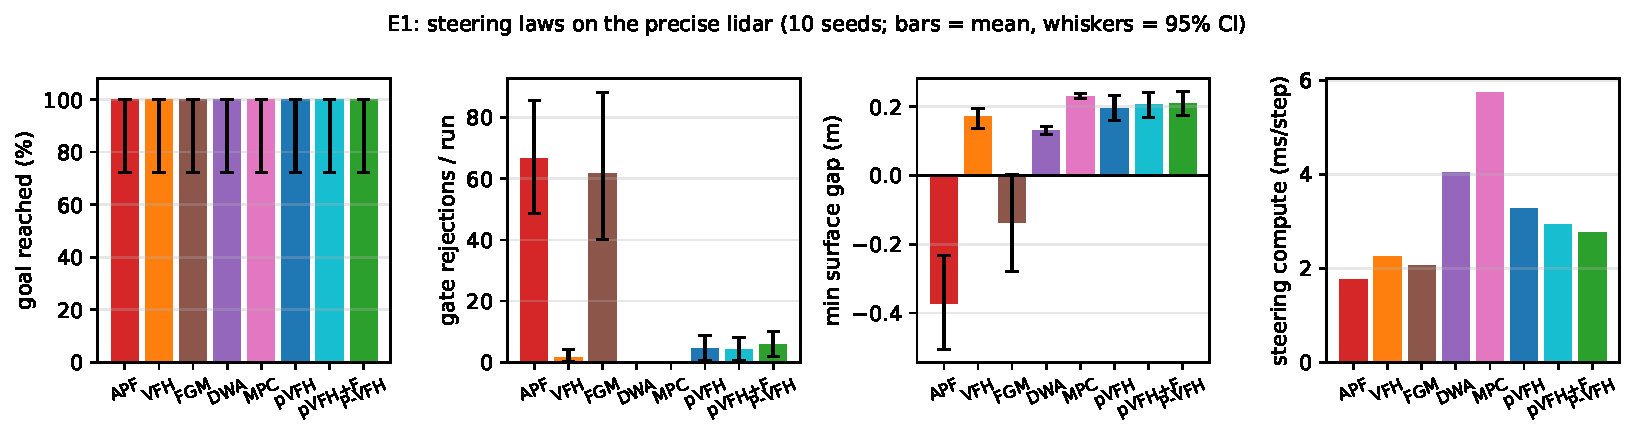
\includegraphics[width=\textwidth]{figures/algo_bars.pdf}
\caption{E1 summary per law: reach rate, gate rejections, minimum surface
gap, steering compute.}
\label{fig:e1bars}
\end{figure}

\begin{figure}[H]
\centering
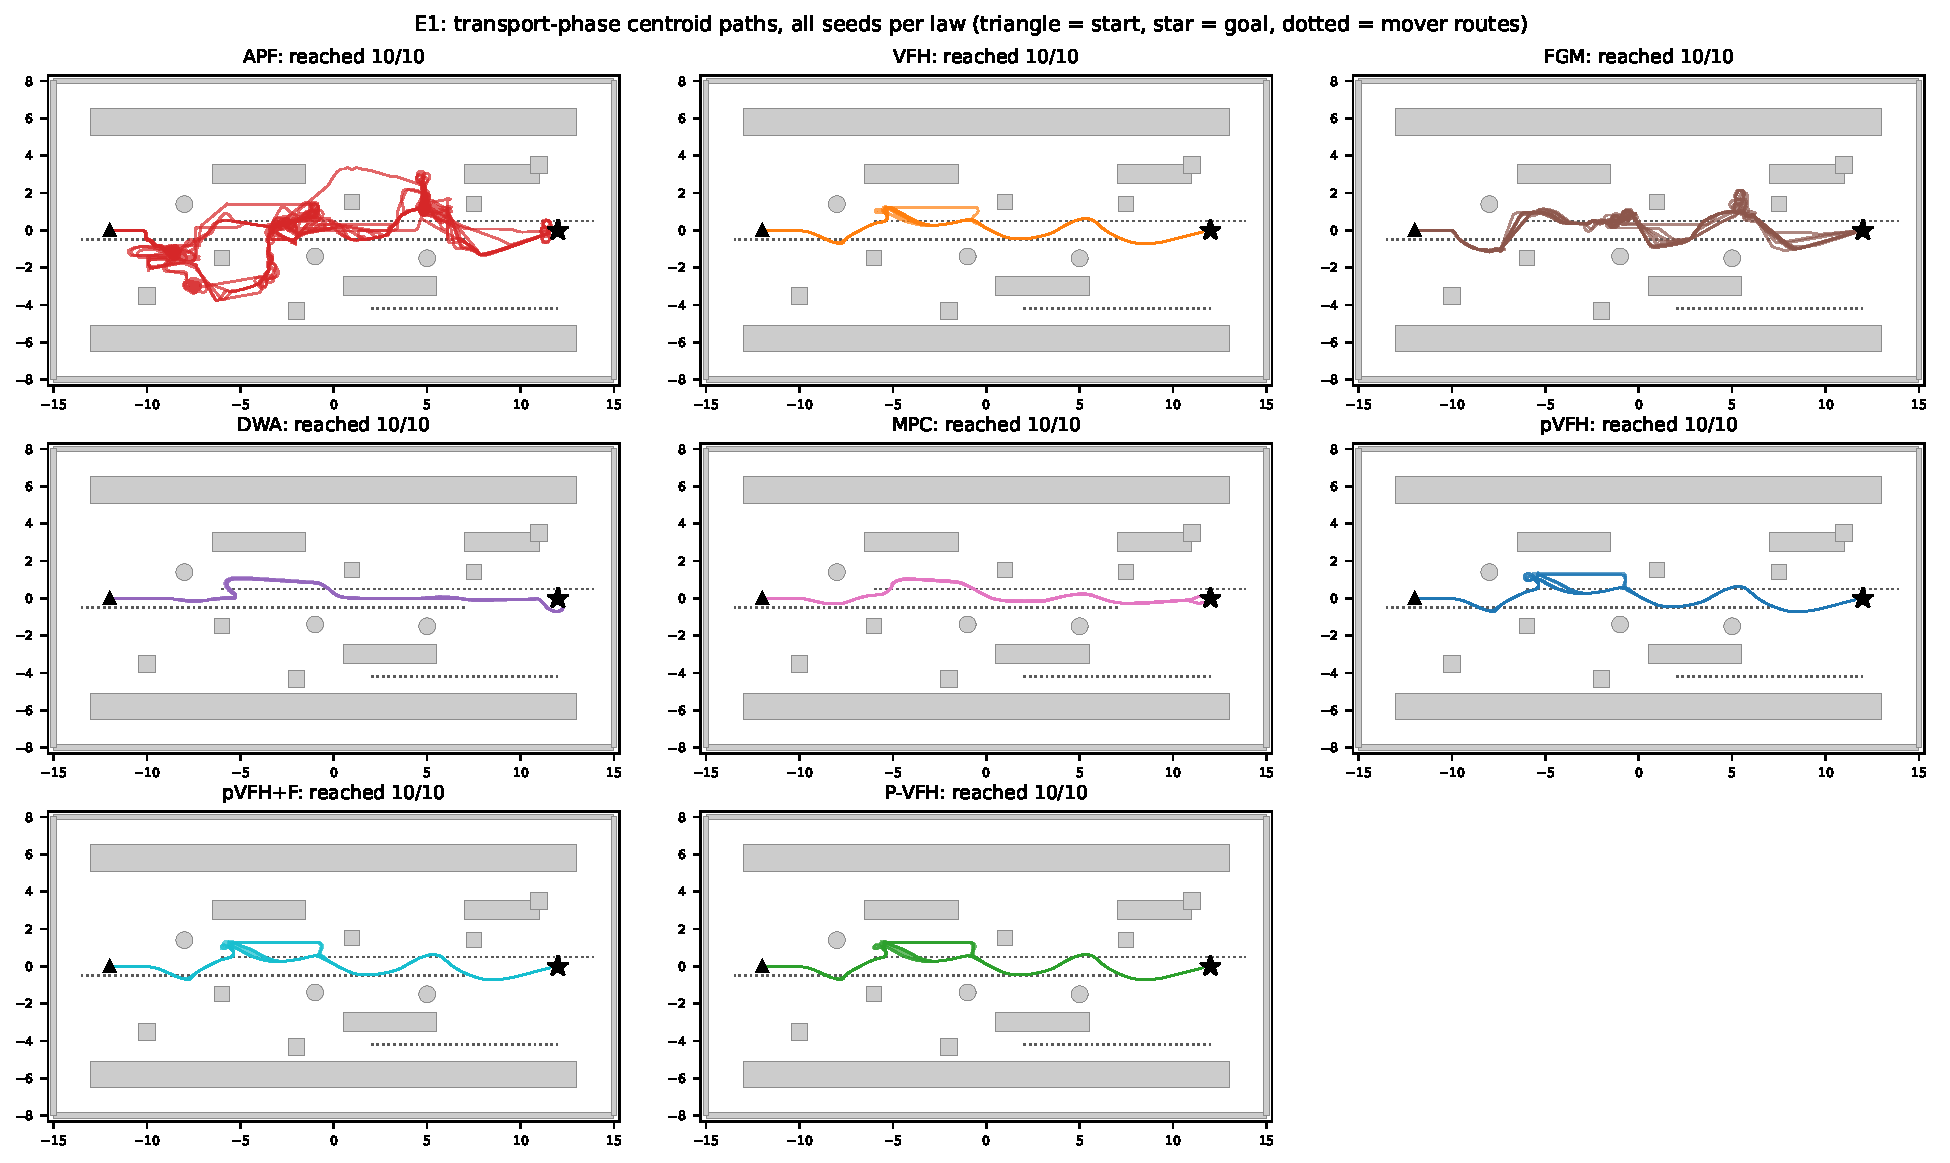
\includegraphics[width=\textwidth]{figures/trajectory_overlays.pdf}
\caption{E1 transport-phase centroid paths on the warehouse map, one panel
per law, every seed overlaid.}
\label{fig:overlays}
\end{figure}

\paragraph{How to read E1.} Start with reach: a law that does not arrive
has no meaningful efficiency. Then read the two safety columns together. A
law with few gate rejections and a healthy gap steered clear by itself; a
law with many rejections arrived only because the supervisor kept refusing
its commands. A law that fails to arrive with \emph{no} rejections is in a
local minimum (the classical APF failure, \S\ref{sec:concept-apf}): it
stopped making progress without ever asking for an unsafe move. In
Fig.~\ref{fig:overlays}, tight bundles mean the law's decisions are
insensitive to the noise realisation; fanned bundles mean they are not.
The compute panel matters only relative to the 100~ms control period.

\subsection{E2 --- noise ablation}
\label{sec:e2}

The central experiment. As $\sigma_0$ grows, a deterministic histogram
thresholds a kernel of the \emph{measured} range, so one outlier can open
or seal a corridor. P-VFH answers with two things: the range filter of
\S\ref{sec:rfilter}, whose gain is set by the sensor model, and the
expected kernel. The ladder \code{pvfh} $\to$ \code{pvfh\_filt} $\to$
\code{pvfh\_prob} separates them. The predictions to test: the filter step
should cut gate rejections and mission time at high $\sigma_0$ and change
nothing at low $\sigma_0$; the kernel step is the open question.

\begin{figure}[H]
\centering
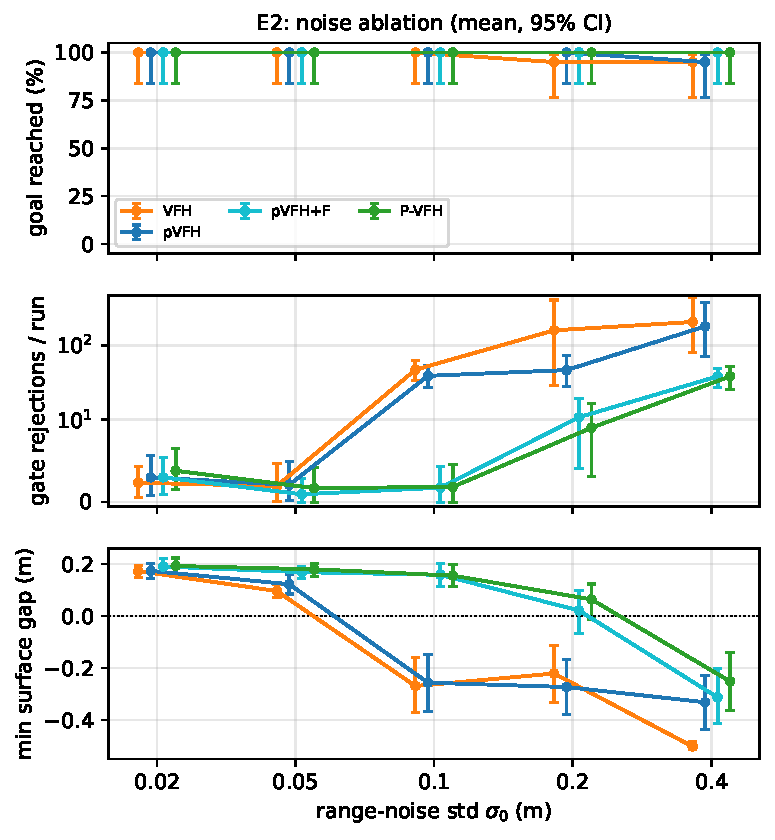
\includegraphics[width=0.74\textwidth]{figures/ablation_noise.pdf}
\caption{E2: reach rate, gate rejections and minimum surface gap against
$\sigma_0$, one line per law (points are dodged horizontally so coincident
intervals stay visible).}
\label{fig:e2}
\end{figure}

% AUTO-GENERATED by matlab/make_paper_figures.py -- do not edit
\begin{table}[H]
\centering\scriptsize
\begin{tabular}{@{}llrrrrrrr@{}}
\toprule
\textbf{Law} & \textbf{$\sigma_0$} & \textbf{Reach} [95\% CI, \%] & \textbf{Gate rej.} & \textbf{Static} & \textbf{Mover} & \textbf{Min gap (m)} [95\% CI] & \textbf{Eff.} & \textbf{Time (s)} \\
\midrule
VFH & 0.02 & 20/20 [84,100] & 2.4 & 0 & 0.0 & 0.17 [0.15,0.19] & 0.90 & 50 \\
VFH & 0.05 & 20/20 [84,100] & 1.9 & 0 & 0.0 & 0.10 [0.07,0.12] & 0.82 & 54 \\
VFH & 0.1 & 20/20 [84,100] & 46.9 & 0 & 26.9 & -0.27 [-0.37,-0.17] & 0.60 & 77 \\
VFH & 0.2 & 19/20 [76,99] & 158.7 & 0 & 14.3 & -0.22 [-0.33,-0.11] & 0.50 & 99 \\
VFH & 0.4 & 19/20 [76,99] & 205.6 & 0 & 39.2 & -0.50 [-0.51,-0.48] & 0.40 & 123 \\
\midrule
pVFH & 0.02 & 20/20 [84,100] & 3.0 & 0 & 0.0 & 0.17 [0.14,0.20] & 0.88 & 51 \\
pVFH & 0.05 & 20/20 [84,100] & 2.1 & 0 & 0.0 & 0.12 [0.08,0.16] & 0.82 & 53 \\
pVFH & 0.1 & 20/20 [84,100] & 38.8 & 0 & 21.8 & -0.26 [-0.36,-0.15] & 0.59 & 77 \\
pVFH & 0.2 & 20/20 [84,100] & 46.3 & 0 & 17.6 & -0.27 [-0.38,-0.17] & 0.50 & 89 \\
pVFH & 0.4 & 19/20 [76,99] & 179.7 & 0 & 36.0 & -0.33 [-0.44,-0.23] & 0.38 & 125 \\
\midrule
pVFH+F & 0.02 & 20/20 [84,100] & 3.0 & 0 & 0.0 & 0.19 [0.16,0.22] & 0.88 & 50 \\
pVFH+F & 0.05 & 20/20 [84,100] & 0.9 & 0 & 0.0 & 0.17 [0.14,0.19] & 0.86 & 51 \\
pVFH+F & 0.1 & 20/20 [84,100] & 1.8 & 0 & 0.0 & 0.16 [0.12,0.20] & 0.83 & 53 \\
pVFH+F & 0.2 & 20/20 [84,100] & 10.8 & 0 & 5.2 & 0.02 [-0.07,0.09] & 0.72 & 62 \\
pVFH+F & 0.4 & 20/20 [84,100] & 38.1 & 0 & 18.8 & -0.31 [-0.42,-0.20] & 0.53 & 84 \\
\midrule
P-VFH & 0.02 & 20/20 [84,100] & 3.8 & 0 & 0.0 & 0.19 [0.16,0.22] & 0.88 & 50 \\
P-VFH & 0.05 & 20/20 [84,100] & 1.7 & 0 & 0.0 & 0.18 [0.15,0.20] & 0.87 & 51 \\
P-VFH & 0.1 & 20/20 [84,100] & 1.9 & 0 & 0.0 & 0.16 [0.11,0.20] & 0.83 & 53 \\
P-VFH & 0.2 & 20/20 [84,100] & 9.0 & 0 & 1.4 & 0.06 [-0.01,0.12] & 0.72 & 63 \\
P-VFH & 0.4 & 20/20 [84,100] & 38.1 & 0 & 18.3 & -0.25 [-0.37,-0.14] & 0.56 & 81 \\
\bottomrule
\end{tabular}
\caption{E2, every cell. Reach: runs reaching the goal, Wilson interval. Gate rej.: mean steps per run in which the safety gate refused the commanded motion. Static: total static-contact steps over the cell (must be 0). Mover: mean steps per run in contact with a mover. Min gap: mean over runs of the per-run minimum surface gap, bootstrap interval. $\dagger$ = legacy pre-fix table, where this column is the old collision-step count.}
\label{tab:e2}
\end{table}


\paragraph{How to read E2.} The three panels share the x-axis. Top: the
fraction of runs that reached the goal --- a drop from 100\% is a law
starting to lose runs. Middle: gate rejections on a symmetric-log axis ---
the count of commands the supervisor refused. Bottom: the margin kept at
the worst moment of the run; the dotted line is contact. The prediction
above is supported only if the P-VFH line is at or above the deterministic
lines in the top and bottom panels and at or below them in the middle one,
with intervals that separate; overlapping intervals mean the experiment
did not resolve a difference at that noise level.

\subsection{Paired analysis}
\label{sec:paired}

\begin{figure}[H]
\centering
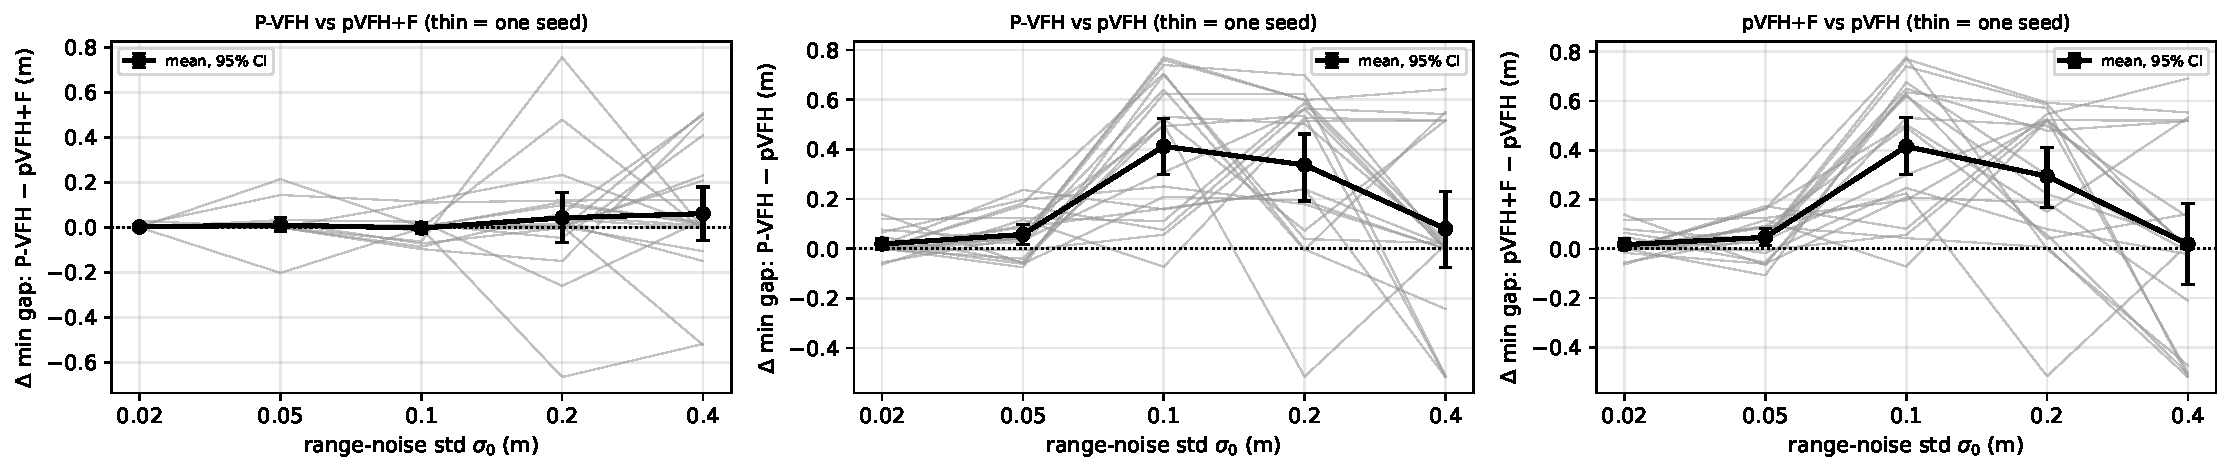
\includegraphics[width=\textwidth]{figures/paired_difference.pdf}
\caption{E2 paired by seed: difference in minimum surface gap per seed
(thin) and mean with 95\% interval (bold), for each step of the ladder:
P-VFH minus \code{pvfh\_filt} (the expected kernel alone), P-VFH minus
\code{pvfh} (filter and kernel), and \code{pvfh\_filt} minus \code{pvfh}
(the filter alone).}
\label{fig:paired}
\end{figure}

% AUTO-GENERATED by matlab/make_paper_figures.py -- do not edit
\begin{table}[H]
\centering\scriptsize
\begin{tabular}{@{}lllrrrrrrr@{}}
\toprule
\textbf{Exp.} & \textbf{World} & \textbf{vs} & $\sigma_0$ & $\Delta$\textbf{gap (m)} [95\% CI] & $p_W$ & $\Delta$\textbf{rej.} [95\% CI] & $p_W$ & \textbf{win/loss} & $p_M$ \\
\midrule
E2 & dynamic & pVFH+F & 0.02 & +0.00 [-0.00,+0.01] & 0.034 & +0.8 [+0.0,+2.4] & 0.180 & 0/0 & -- \\
E2 & dynamic & pVFH+F & 0.05 & +0.01 [-0.02,+0.04] & 0.152 & +0.8 [+0.0,+2.2] & 0.180 & 0/0 & -- \\
E2 & dynamic & pVFH+F & 0.1 & -0.00 [-0.03,+0.02] & 0.948 & +0.1 [+0.0,+0.3] & 0.317 & 0/0 & -- \\
E2 & dynamic & pVFH+F & 0.2 & +0.04 [-0.07,+0.16] & 0.165 & -1.8 [-11.0,+8.2] & 0.449 & 0/0 & -- \\
E2 & dynamic & pVFH+F & 0.4 & +0.06 [-0.07,+0.18] & 0.245 & +0.1 [-14.5,+14.5] & 0.896 & 0/0 & -- \\
E2 & dynamic & pVFH & 0.02 & +0.02 [-0.00,+0.04] & 0.076 & +0.8 [-2.0,+3.6] & 0.498 & 0/0 & -- \\
E2 & dynamic & pVFH & 0.05 & +0.06 [+0.02,+0.10] & 0.033 & -0.4 [-3.0,+2.2] & 0.389 & 0/0 & -- \\
E2 & dynamic & pVFH & 0.1 & +0.41 [+0.29,+0.53] & $<$0.001 & -36.9 [-49.5,-25.2] & $<$0.001 & 0/0 & -- \\
E2 & dynamic & pVFH & 0.2 & +0.34 [+0.19,+0.46] & $<$0.001 & -37.3 [-63.1,-17.9] & $<$0.001 & 0/0 & -- \\
E2 & dynamic & pVFH & 0.4 & +0.08 [-0.08,+0.24] & 0.083 & -141.6 [-346.9,-25.9] & 0.002 & 1/0 & 1.000 \\
E2 & dynamic & VFH & 0.02 & +0.02 [-0.01,+0.05] & 0.133 & +1.4 [-1.6,+4.4] & 0.297 & 0/0 & -- \\
E2 & dynamic & VFH & 0.05 & +0.08 [+0.05,+0.12] & $<$0.001 & -0.2 [-2.6,+2.4] & 0.596 & 0/0 & -- \\
E2 & dynamic & VFH & 0.1 & +0.43 [+0.30,+0.54] & $<$0.001 & -45.0 [-60.4,-31.3] & $<$0.001 & 0/0 & -- \\
E2 & dynamic & VFH & 0.2 & +0.29 [+0.15,+0.42] & $<$0.001 & -149.7 [-401.4,-17.1] & 0.001 & 1/0 & 1.000 \\
E2 & dynamic & VFH & 0.4 & +0.25 [+0.13,+0.37] & $<$0.001 & -167.4 [-407.6,-39.9] & $<$0.001 & 1/0 & 1.000 \\
E7 & maze & pVFH+F & 0.02 & -0.00 [-0.00,+0.00] & 1.000 & +0.0 [+0.0,+0.0] & -- & 0/0 & -- \\
E7 & maze & pVFH+F & 0.2 & -0.00 [-0.00,+0.00] & 1.000 & +0.0 [+0.0,+0.0] & -- & 0/0 & -- \\
E7 & maze & pVFH & 0.02 & -0.00 [-0.00,+0.00] & 0.064 & +0.0 [+0.0,+0.0] & -- & 0/0 & -- \\
E7 & maze & pVFH & 0.2 & +0.16 [+0.12,+0.20] & 0.002 & -2.2 [-5.7,-0.2] & 0.125 & 0/0 & -- \\
E7 & maze & VFH & 0.02 & -0.00 [-0.00,+0.00] & 0.064 & +0.0 [+0.0,+0.0] & -- & 0/0 & -- \\
E7 & maze & VFH & 0.2 & +0.14 [+0.09,+0.19] & 0.002 & -0.5 [-1.0,+0.0] & 0.250 & 0/0 & -- \\
E7 & plaza & pVFH+F & 0.02 & +0.01 [-0.15,+0.21] & 1.000 & -1.4 [-37.9,+25.4] & 0.875 & 0/0 & -- \\
E7 & plaza & pVFH+F & 0.2 & -0.05 [-0.14,+0.02] & 0.770 & +8.3 [-5.9,+23.2] & 0.461 & 0/0 & -- \\
E7 & plaza & pVFH & 0.02 & +0.00 [-0.30,+0.30] & 1.000 & -9.3 [-47.0,+26.5] & 0.367 & 0/0 & -- \\
E7 & plaza & pVFH & 0.2 & -0.00 [-0.15,+0.14] & 1.000 & +7.1 [-17.1,+32.9] & 0.625 & 0/0 & -- \\
E7 & plaza & VFH & 0.02 & +0.04 [-0.21,+0.28] & 0.432 & +2.2 [-30.6,+34.4] & 0.945 & 0/0 & -- \\
E7 & plaza & VFH & 0.2 & -0.02 [-0.18,+0.15] & 1.000 & +5.4 [-25.6,+33.4] & 0.770 & 0/0 & -- \\
E13 & 10 random layouts & pVFH+F & 0.02 & +0.00 [-0.00,+0.01] & 0.073 & -66.6 [-196.8,+0.0] & 0.104 & 1/0 & 1.000 \\
E13 & 10 random layouts & pVFH+F & 0.2 & -0.01 [-0.05,+0.04] & 0.209 & +1.6 [-4.7,+7.8] & 0.480 & 0/0 & -- \\
E13 & 10 random layouts & pVFH & 0.02 & +0.02 [-0.01,+0.07] & 0.152 & +6.7 [-5.7,+26.3] & 0.683 & 0/0 & -- \\
E13 & 10 random layouts & pVFH & 0.2 & +0.01 [-0.05,+0.09] & 0.490 & -99.4 [-253.3,-9.0] & 0.047 & 1/0 & 1.000 \\
E13 & 10 random layouts & VFH & 0.02 & +0.09 [+0.02,+0.17] & 0.584 & +9.8 [-10.0,+44.7] & 0.033 & 0/0 & -- \\
E13 & 10 random layouts & VFH & 0.2 & +0.12 [+0.04,+0.19] & 0.043 & -182.3 [-434.5,-14.6] & $<$0.001 & 2/0 & 0.500 \\
\bottomrule
\end{tabular}
\caption{Paired-seed tests, P-VFH minus the named deterministic law (positive $\Delta$gap and negative $\Delta$rej.\ favour P-VFH). $p_W$: two-sided Wilcoxon signed-rank on the per-seed differences; win/loss: seeds where only P-VFH / only the baseline reached the goal, $p_M$: exact McNemar (binomial) test on those discordant pairs. Intervals are percentile bootstrap. No multiplicity correction is applied; read the $p$-values with the number of rows in mind.}
\label{tab:stats}
\end{table}


\paragraph{How to read the paired results.} A point above zero favours the
first-named law at that noise level \emph{if} its interval excludes zero.
The left panel is the test of the expected kernel on its own; the right
panel is the test of the filter on its own. Whichever panel sits at zero
names the component that is not contributing. The thin lines show how
much individual seeds disagree; a mean carried by one or two seeds is weak
evidence however large it is. In Table~\ref{tab:stats}, the Wilcoxon
$p$-value addresses the size of the difference and the McNemar $p$-value
addresses reach; with this many rows, isolated values near 0.05 should not
be read as findings.

\subsection{E3 --- beam sweep}
\label{sec:e3}

\begin{figure}[H]
\centering
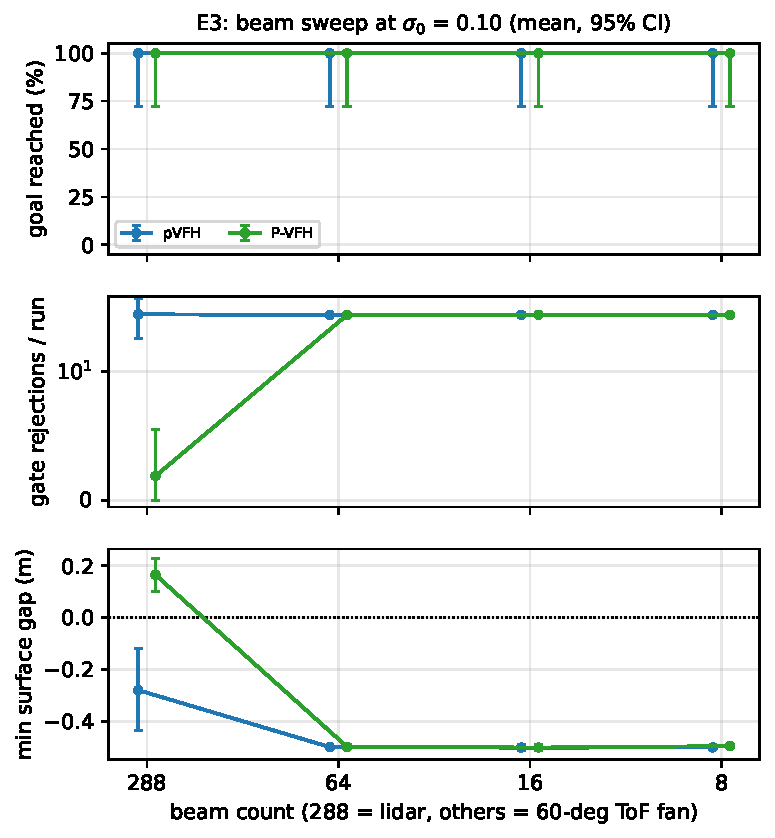
\includegraphics[width=0.74\textwidth]{figures/sweep_tof.pdf}
\caption{E3: the same three metrics against beam count at
$\sigma_0 = 0.10$~m (288 = lidar; 64, 16, 8 = $60^\circ$ body-fixed ToF
fan).}
\label{fig:e3}
\end{figure}

% AUTO-GENERATED by matlab/make_paper_figures.py -- do not edit
\begin{table}[H]
\centering\scriptsize
\begin{tabular}{@{}llrrrrrrr@{}}
\toprule
\textbf{Law} & \textbf{Sensor} & \textbf{Reach} [95\% CI, \%] & \textbf{Gate rej.} & \textbf{Static} & \textbf{Mover} & \textbf{Min gap (m)} [95\% CI] & \textbf{Eff.} & \textbf{Time (s)} \\
\midrule
pVFH & lidar-288 & 10/10 [72,100] & 30.8 & 0 & 16.1 & -0.28 [-0.44,-0.12] & 0.59 & 76 \\
pVFH & tof-64 & 10/10 [72,100] & 30.4 & 0 & 28.9 & -0.50 [-0.51,-0.49] & 1.00 & 48 \\
pVFH & tof-16 & 10/10 [72,100] & 30.5 & 0 & 29.0 & -0.50 [-0.51,-0.49] & 1.00 & 48 \\
pVFH & tof-8 & 10/10 [72,100] & 30.5 & 0 & 29.0 & -0.50 [-0.51,-0.49] & 1.00 & 48 \\
\midrule
P-VFH & lidar-288 & 10/10 [72,100] & 1.9 & 0 & 0.0 & 0.16 [0.10,0.22] & 0.83 & 53 \\
P-VFH & tof-64 & 10/10 [72,100] & 30.4 & 0 & 28.9 & -0.50 [-0.50,-0.49] & 1.00 & 48 \\
P-VFH & tof-16 & 10/10 [72,100] & 30.5 & 0 & 29.0 & -0.50 [-0.51,-0.49] & 1.00 & 48 \\
P-VFH & tof-8 & 10/10 [72,100] & 30.4 & 0 & 28.9 & -0.50 [-0.50,-0.49] & 1.00 & 48 \\
\bottomrule
\end{tabular}
\caption{E3. Reach: runs reaching the goal, Wilson interval. Gate rej.: mean steps per run in which the safety gate refused the commanded motion. Static: total static-contact steps over the cell (must be 0). Mover: mean steps per run in contact with a mover. Min gap: mean over runs of the per-run minimum surface gap, bootstrap interval. $\dagger$ = legacy pre-fix table, where this column is the old collision-step count.}
\label{tab:e3}
\end{table}


\paragraph{How to read E3.} Two things change between 288 and 64 beams ---
the fan narrows from $360^\circ$ to $60^\circ$ and the noise becomes
range-dependent --- so that step is a change of sensor, not only of
resolution; the 64~$\to$~16~$\to$~8 steps isolate resolution. A flat reach
line with a falling gap is the early warning: the law still arrives but
with less room. Watch the mover-contact column: a narrow forward fan cannot
see traffic approaching from the side or rear, and no steering law can
avoid what its sensor does not report.

\subsection{E4 --- formation shapes}
\label{sec:e4}

\begin{figure}[H]
\centering
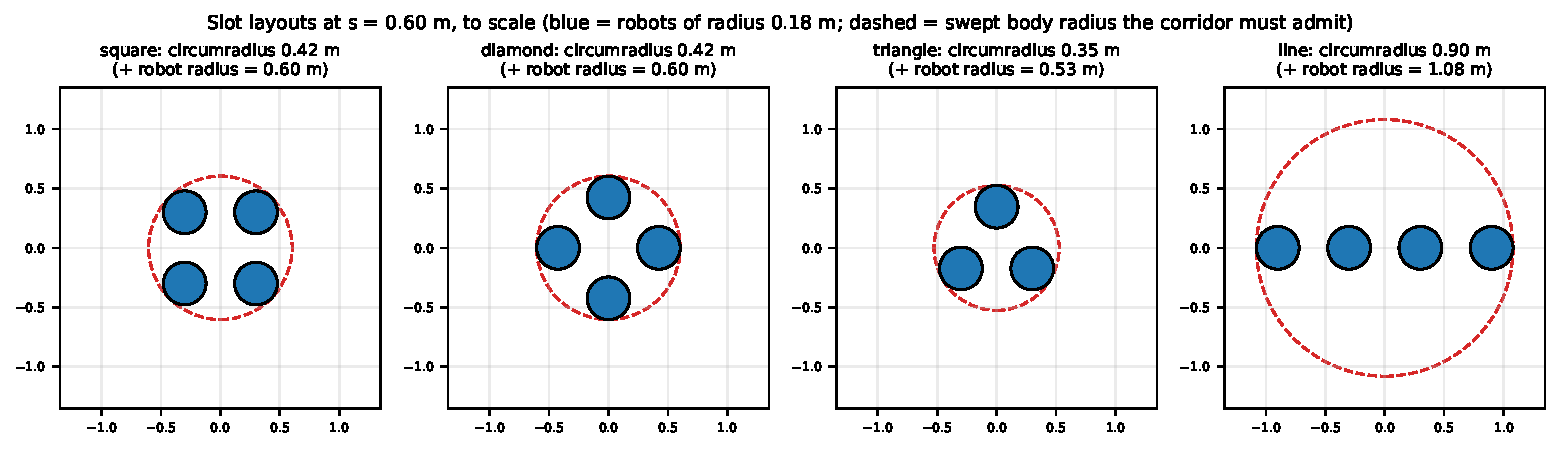
\includegraphics[width=0.95\textwidth]{figures/formation_sketch.pdf}
\caption{The four slot layouts at the E4/E5 spacing, to scale.}
\label{fig:fsketch}
\end{figure}

% AUTO-GENERATED by matlab/make_paper_figures.py -- do not edit
\begin{table}[H]
\centering\scriptsize
\begin{tabular}{@{}lrrrrrrr@{}}
\toprule
\textbf{Shape} & \textbf{Reach} [95\% CI, \%] & \textbf{Gate rej.} & \textbf{Static} & \textbf{Mover} & \textbf{Min gap (m)} [95\% CI] & \textbf{Eff.} & \textbf{Time (s)} \\
\midrule
square & 10/10 [72,100] & 0.0 & 0 & 0.0 & 0.62 [0.61,0.62] & 0.91 & 49 \\
diamond & 10/10 [72,100] & 0.0 & 0 & 0.0 & 0.49 [0.49,0.49] & 0.91 & 48 \\
triangle & 10/10 [72,100] & 0.0 & 0 & 0.0 & 0.58 [0.58,0.58] & 0.92 & 49 \\
line & 10/10 [72,100] & 10.7 & 0 & 1.8 & -0.02 [-0.11,0.03] & 0.52 & 84 \\
\bottomrule
\end{tabular}
\caption{E4. Reach: runs reaching the goal, Wilson interval. Gate rej.: mean steps per run in which the safety gate refused the commanded motion. Static: total static-contact steps over the cell (must be 0). Mover: mean steps per run in contact with a mover. Min gap: mean over runs of the per-run minimum surface gap, bootstrap interval. $\dagger$ = legacy pre-fix table, where this column is the old collision-step count.}
\label{tab:e4}
\end{table}


\begin{figure}[H]
\centering
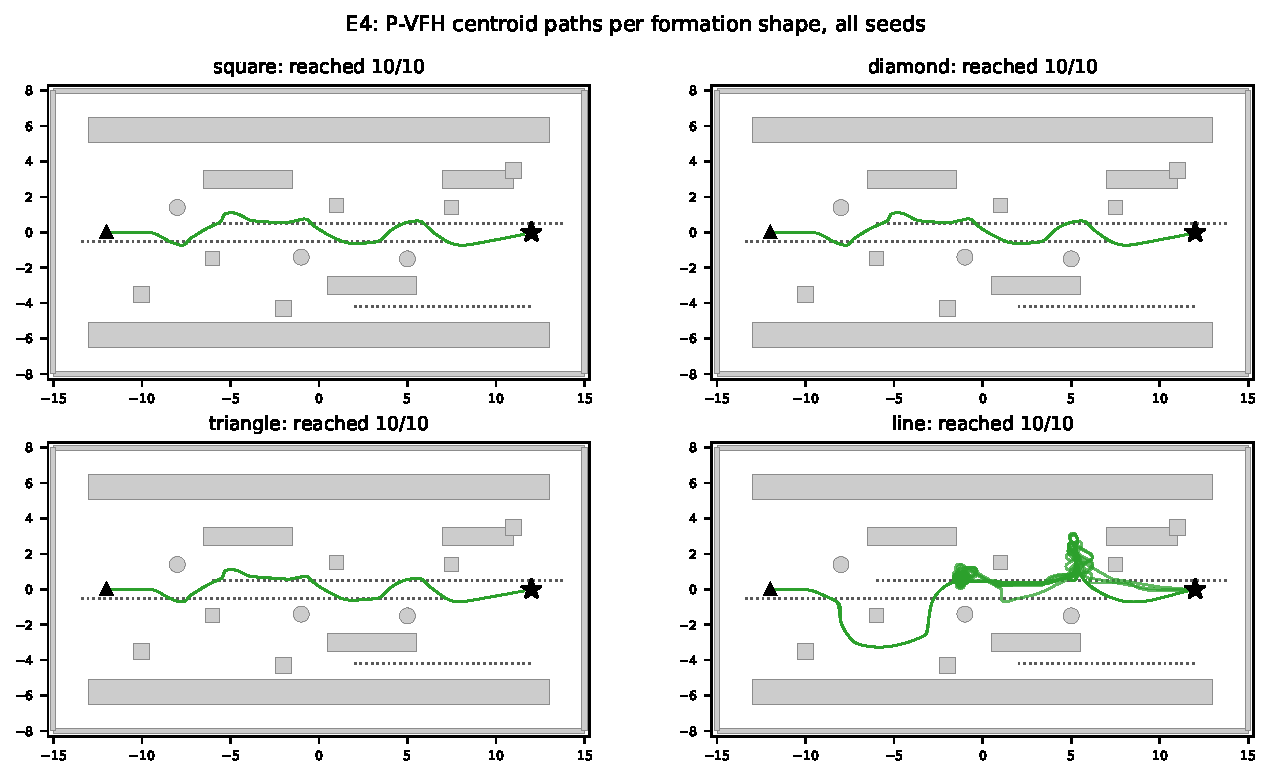
\includegraphics[width=\textwidth]{figures/formation_trails.pdf}
\caption{E4: P-VFH centroid paths for each shape, every seed.}
\label{fig:ftrails}
\end{figure}

\paragraph{How to read E4.} The corridor bottleneck is a half-width of
$1.22$~m. Square, diamond and triangle have swept radii well below it and
can turn anywhere. The line is different in kind: its swept radius also
fits, but it is a $2.16$~m-long body (four robots at $0.60$~m plus two
radii) that must \emph{rotate} to follow the chicane, and a rotation that
is blocked is a pivot the mission layer has to resolve. Expect the line to
be the slow shape; whether it is also a failing one is what the table
reports.

\subsection{E5 --- formation $\times$ steering law}
\label{sec:e5}

\begin{figure}[H]
\centering
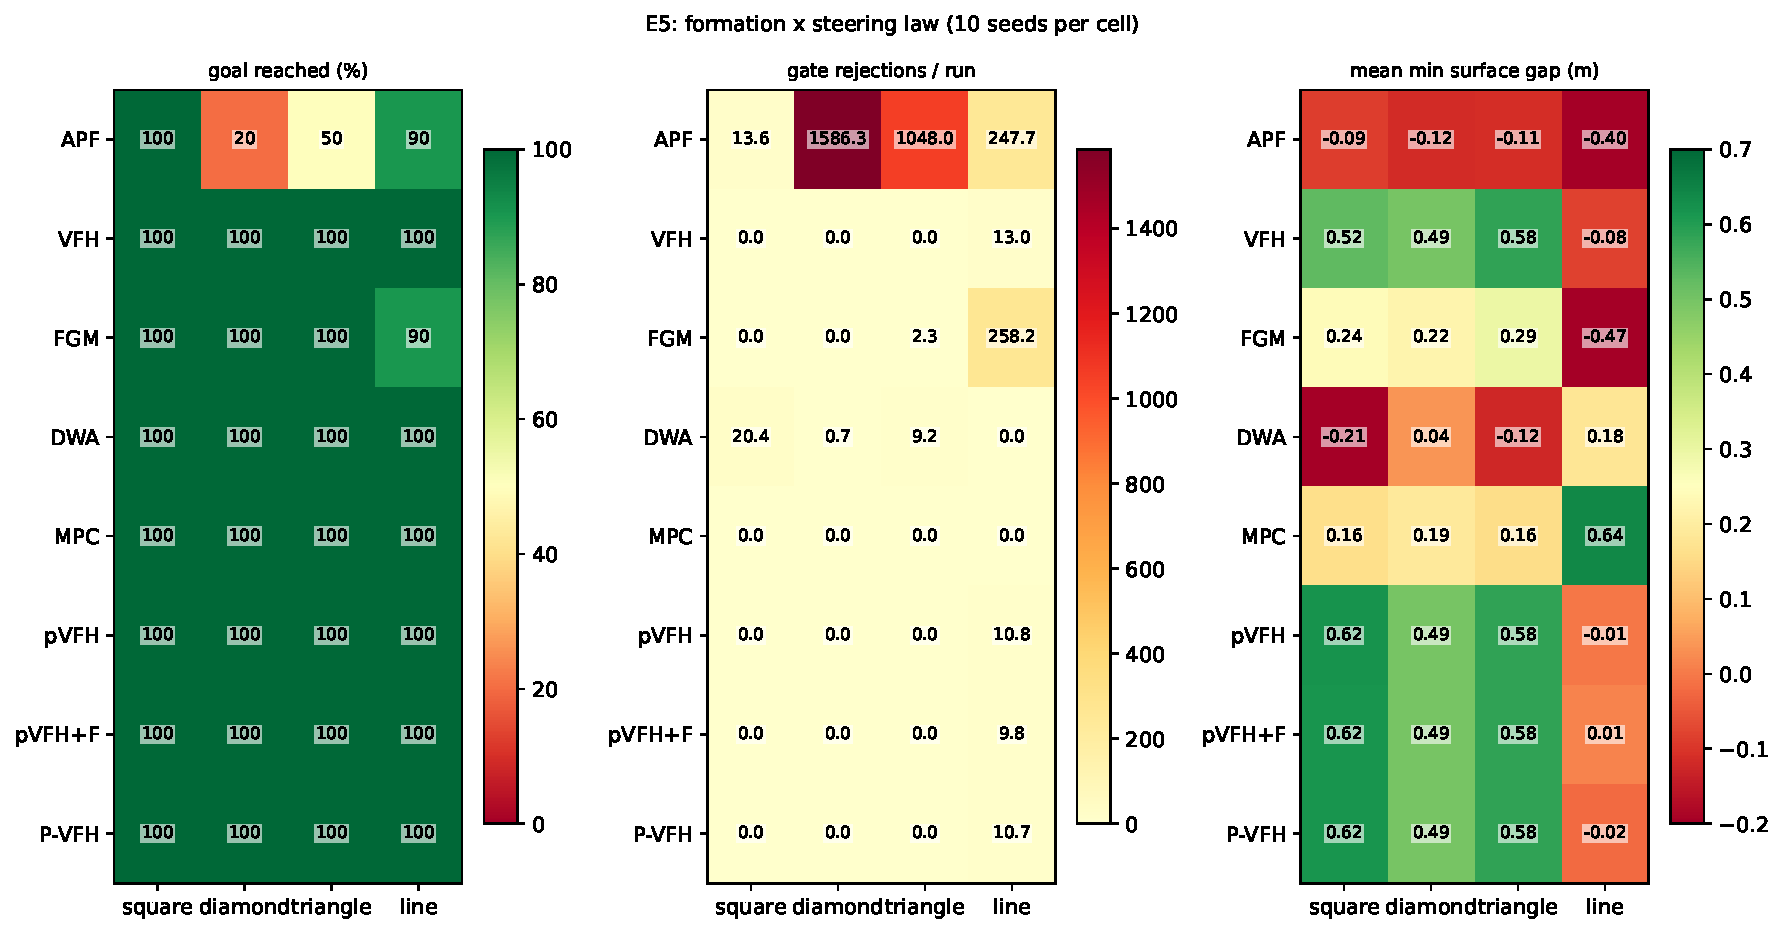
\includegraphics[width=\textwidth]{figures/e5_heatmap.pdf}
\caption{E5: reach rate, gate rejections and mean minimum surface gap per
(law, shape) cell.}
\label{fig:e5heat}
\end{figure}

% AUTO-GENERATED by matlab/make_paper_figures.py -- do not edit
\begin{table}[H]
\centering\scriptsize
\begin{tabular}{@{}llrrrrrrr@{}}
\toprule
\textbf{Law} & \textbf{Shape} & \textbf{Reach} [95\% CI, \%] & \textbf{Gate rej.} & \textbf{Static} & \textbf{Mover} & \textbf{Min gap (m)} [95\% CI] & \textbf{Eff.} & \textbf{Time (s)} \\
\midrule
APF & square & 10/10 [72,100] & 13.6 & 0 & 4.2 & -0.09 [-0.24,0.02] & 0.43 & 100 \\
APF & diamond & 2/10 [6,51] & 1586.3 & 0 & 6.1 & -0.12 [-0.26,0.00] & 0.23 & 268 \\
APF & triangle & 5/10 [24,76] & 1048.0 & 0 & 7.9 & -0.11 [-0.29,0.07] & 0.31 & 205 \\
APF & line & 9/10 [60,98] & 247.7 & 0 & 32.9 & -0.40 [-0.46,-0.35] & 0.31 & 150 \\
\midrule
VFH & square & 10/10 [72,100] & 0.0 & 0 & 0.0 & 0.52 [0.52,0.53] & 0.92 & 49 \\
VFH & diamond & 10/10 [72,100] & 0.0 & 0 & 0.0 & 0.49 [0.49,0.50] & 0.92 & 48 \\
VFH & triangle & 10/10 [72,100] & 0.0 & 0 & 0.0 & 0.58 [0.58,0.58] & 0.92 & 49 \\
VFH & line & 10/10 [72,100] & 13.0 & 0 & 4.1 & -0.08 [-0.23,0.02] & 0.51 & 85 \\
\midrule
FGM & square & 10/10 [72,100] & 0.0 & 0 & 0.0 & 0.24 [0.22,0.27] & 0.89 & 50 \\
FGM & diamond & 10/10 [72,100] & 0.0 & 0 & 0.0 & 0.22 [0.20,0.24] & 0.90 & 49 \\
FGM & triangle & 10/10 [72,100] & 2.3 & 0 & 2.0 & 0.29 [0.12,0.40] & 0.85 & 53 \\
FGM & line & 9/10 [60,98] & 258.2 & 0 & 30.2 & -0.47 [-0.49,-0.44] & 0.64 & 97 \\
\midrule
DWA & square & 10/10 [72,100] & 20.4 & 0 & 17.8 & -0.21 [-0.23,-0.19] & 0.96 & 51 \\
DWA & diamond & 10/10 [72,100] & 0.7 & 0 & 0.0 & 0.04 [0.03,0.04] & 0.96 & 49 \\
DWA & triangle & 10/10 [72,100] & 9.2 & 0 & 5.9 & -0.12 [-0.18,-0.07] & 0.97 & 50 \\
DWA & line & 10/10 [72,100] & 0.0 & 0 & 0.0 & 0.18 [0.16,0.19] & 0.91 & 51 \\
\midrule
MPC & square & 10/10 [72,100] & 0.0 & 0 & 0.0 & 0.16 [0.16,0.17] & 0.98 & 47 \\
MPC & diamond & 10/10 [72,100] & 0.0 & 0 & 0.0 & 0.19 [0.18,0.20] & 0.98 & 46 \\
MPC & triangle & 10/10 [72,100] & 0.0 & 0 & 0.0 & 0.16 [0.15,0.17] & 0.98 & 47 \\
MPC & line & 10/10 [72,100] & 0.0 & 0 & 0.0 & 0.64 [0.61,0.66] & 0.96 & 47 \\
\midrule
pVFH & square & 10/10 [72,100] & 0.0 & 0 & 0.0 & 0.62 [0.61,0.62] & 0.91 & 49 \\
pVFH & diamond & 10/10 [72,100] & 0.0 & 0 & 0.0 & 0.49 [0.49,0.50] & 0.92 & 48 \\
pVFH & triangle & 10/10 [72,100] & 0.0 & 0 & 0.0 & 0.58 [0.58,0.58] & 0.92 & 48 \\
pVFH & line & 10/10 [72,100] & 10.8 & 0 & 2.1 & -0.01 [-0.13,0.07] & 0.50 & 86 \\
\midrule
pVFH+F & square & 10/10 [72,100] & 0.0 & 0 & 0.0 & 0.62 [0.61,0.62] & 0.91 & 49 \\
pVFH+F & diamond & 10/10 [72,100] & 0.0 & 0 & 0.0 & 0.49 [0.49,0.49] & 0.91 & 48 \\
pVFH+F & triangle & 10/10 [72,100] & 0.0 & 0 & 0.0 & 0.58 [0.58,0.58] & 0.92 & 49 \\
pVFH+F & line & 10/10 [72,100] & 9.8 & 0 & 0.1 & 0.01 [-0.04,0.05] & 0.50 & 86 \\
\midrule
P-VFH & square & 10/10 [72,100] & 0.0 & 0 & 0.0 & 0.62 [0.61,0.62] & 0.91 & 49 \\
P-VFH & diamond & 10/10 [72,100] & 0.0 & 0 & 0.0 & 0.49 [0.49,0.49] & 0.91 & 48 \\
P-VFH & triangle & 10/10 [72,100] & 0.0 & 0 & 0.0 & 0.58 [0.58,0.58] & 0.92 & 49 \\
P-VFH & line & 10/10 [72,100] & 10.7 & 0 & 1.8 & -0.02 [-0.11,0.03] & 0.52 & 84 \\
\bottomrule
\end{tabular}
\caption{E5, every cell. Reach: runs reaching the goal, Wilson interval. Gate rej.: mean steps per run in which the safety gate refused the commanded motion. Static: total static-contact steps over the cell (must be 0). Mover: mean steps per run in contact with a mover. Min gap: mean over runs of the per-run minimum surface gap, bootstrap interval. $\dagger$ = legacy pre-fix table, where this column is the old collision-step count.}
\label{tab:e5}
\end{table}


\begin{figure}[H]
\centering
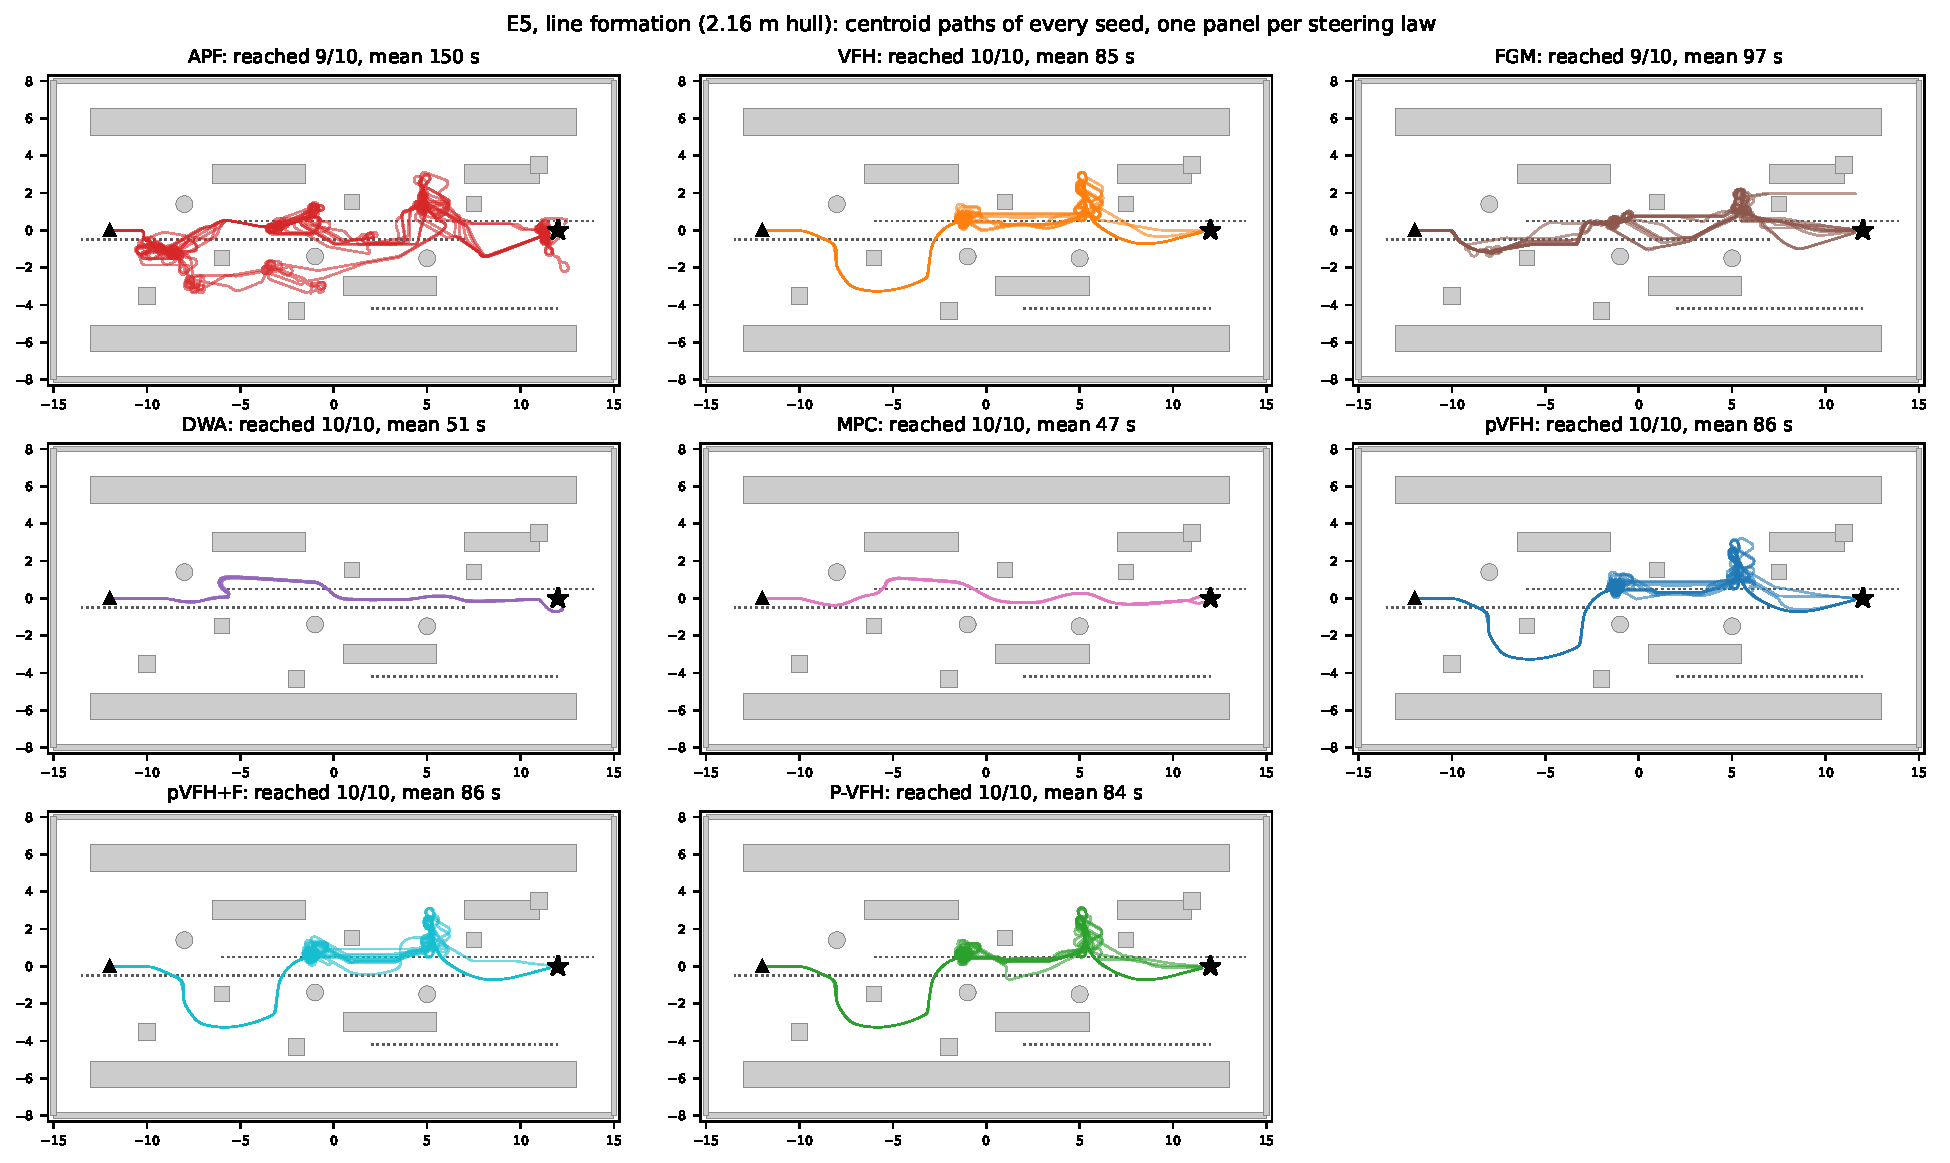
\includegraphics[width=\textwidth]{figures/e5_line_anatomy.pdf}
\caption{E5, line formation: every seed's path, one panel per law.}
\label{fig:e5anatomy}
\end{figure}

\begin{figure}[H]
\centering
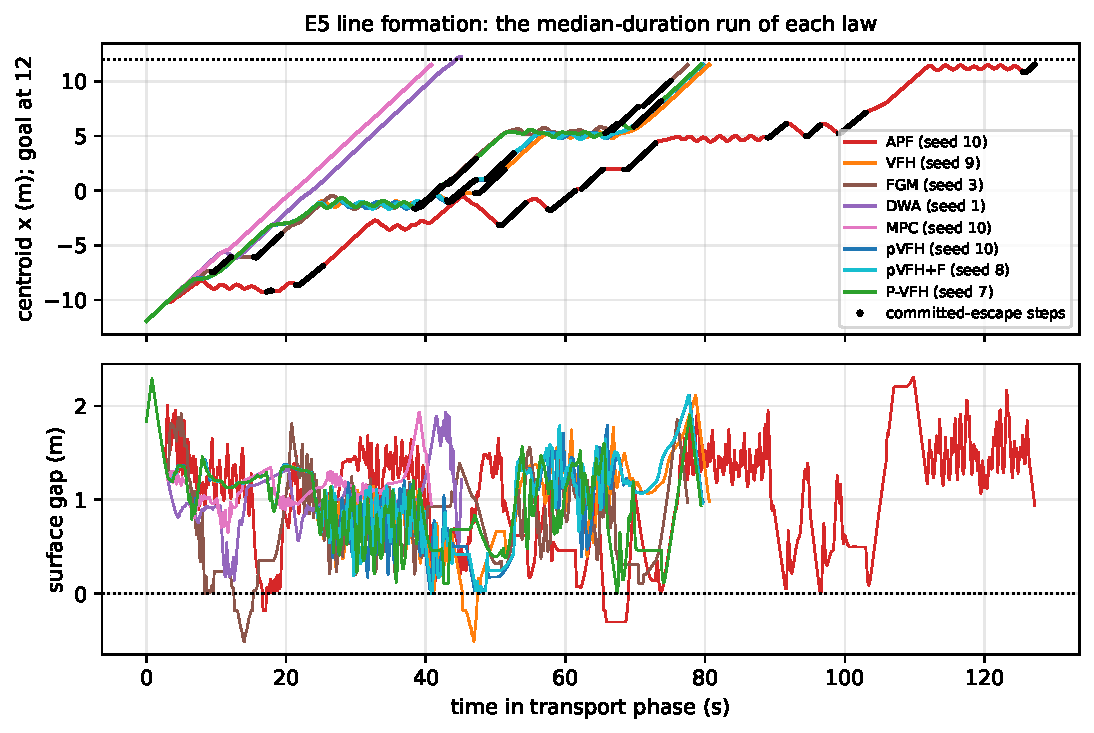
\includegraphics[width=0.85\textwidth]{figures/e5_stall_timeseries.pdf}
\caption{E5, line formation: progress and surface gap over time for the
median-duration run of each law. Black dots mark steps taken under a
committed escape.}
\label{fig:e5stall}
\end{figure}

\paragraph{How to read E5.} Read the heatmaps in two directions.
\emph{Across a row} (fixed law): does the shape matter to this law?
\emph{Down a column} (fixed shape): does the law matter for this shape? A
column in which some cells fail and others do not is an \emph{interaction}
--- the effect of the law depends on the shape --- which neither E1 nor E4
can show. In the time series, a flat stretch of the progress trace is a
stall: if the gap trace below it is near zero the body is jammed against
something; if the gap is comfortably positive it is a pivot that either
the steering law or a committed escape (black dots) must end. The run for
each law is chosen by a rule (median mission time), not by hand.

\subsection{E6 --- matched sensor comparison}
\label{sec:e6}

\begin{figure}[H]
\centering
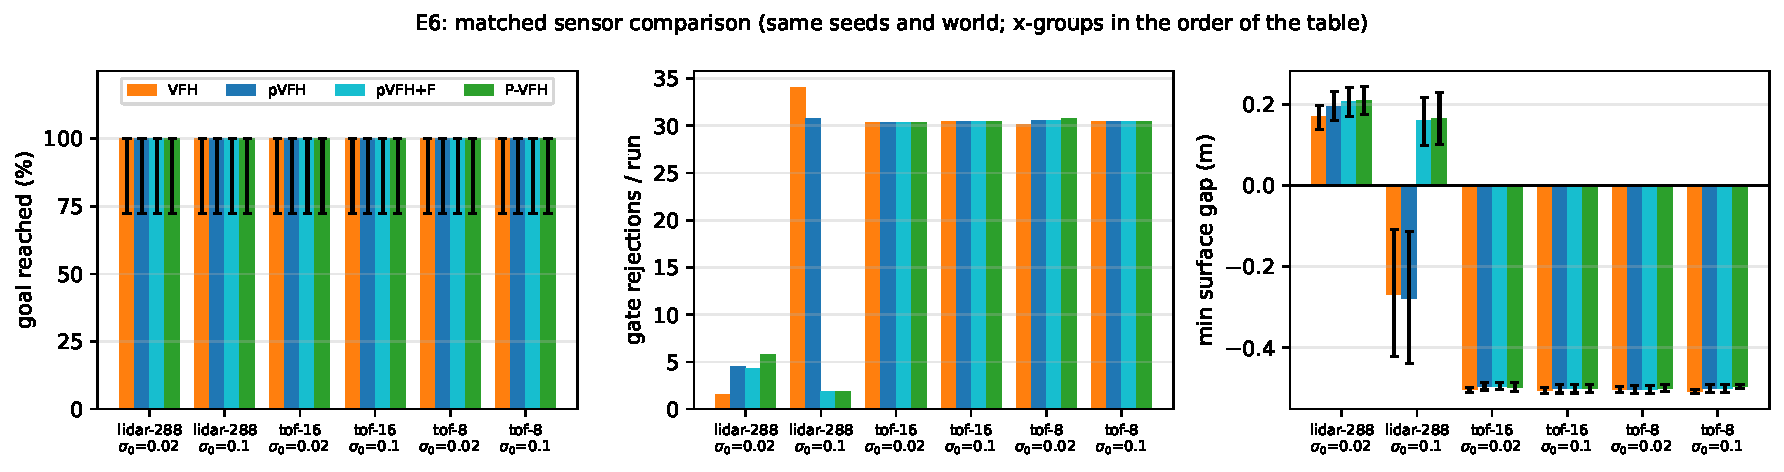
\includegraphics[width=\textwidth]{figures/e6_sensor.pdf}
\caption{E6: reach, gate rejections and gap by sensor configuration and
law.}
\label{fig:e6}
\end{figure}

% AUTO-GENERATED by matlab/make_paper_figures.py -- do not edit
\begin{table}[H]
\centering\scriptsize
\begin{tabular}{@{}lllrrrrrrr@{}}
\toprule
\textbf{Sensor} & \textbf{$\sigma_0$} & \textbf{Law} & \textbf{Reach} [95\% CI, \%] & \textbf{Gate rej.} & \textbf{Static} & \textbf{Mover} & \textbf{Min gap (m)} [95\% CI] & \textbf{Eff.} & \textbf{Time (s)} \\
\midrule
lidar-288 & 0.02 & VFH & 10/10 [72,100] & 1.6 & 0 & 0.0 & 0.17 [0.14,0.20] & 0.90 & 49 \\
lidar-288 & 0.02 & pVFH & 10/10 [72,100] & 4.5 & 0 & 0.0 & 0.19 [0.16,0.23] & 0.89 & 50 \\
lidar-288 & 0.02 & pVFH+F & 10/10 [72,100] & 4.3 & 0 & 0.0 & 0.21 [0.17,0.24] & 0.89 & 50 \\
lidar-288 & 0.02 & P-VFH & 10/10 [72,100] & 5.8 & 0 & 0.0 & 0.21 [0.18,0.24] & 0.89 & 50 \\
lidar-288 & 0.1 & VFH & 10/10 [72,100] & 34.1 & 0 & 15.3 & -0.27 [-0.42,-0.11] & 0.60 & 76 \\
lidar-288 & 0.1 & pVFH & 10/10 [72,100] & 30.8 & 0 & 16.1 & -0.28 [-0.43,-0.12] & 0.59 & 76 \\
lidar-288 & 0.1 & pVFH+F & 10/10 [72,100] & 1.9 & 0 & 0.0 & 0.16 [0.10,0.22] & 0.83 & 53 \\
lidar-288 & 0.1 & P-VFH & 10/10 [72,100] & 1.9 & 0 & 0.0 & 0.16 [0.10,0.23] & 0.83 & 53 \\
\midrule
tof-16 & 0.02 & VFH & 10/10 [72,100] & 30.3 & 0 & 29.0 & -0.50 [-0.51,-0.50] & 1.00 & 48 \\
tof-16 & 0.02 & pVFH & 10/10 [72,100] & 30.3 & 0 & 28.9 & -0.50 [-0.50,-0.49] & 1.00 & 48 \\
tof-16 & 0.02 & pVFH+F & 10/10 [72,100] & 30.3 & 0 & 28.9 & -0.50 [-0.50,-0.49] & 1.00 & 48 \\
tof-16 & 0.02 & P-VFH & 10/10 [72,100] & 30.3 & 0 & 28.9 & -0.50 [-0.51,-0.49] & 1.00 & 48 \\
tof-16 & 0.1 & VFH & 10/10 [72,100] & 30.4 & 0 & 29.0 & -0.51 [-0.51,-0.50] & 1.00 & 48 \\
tof-16 & 0.1 & pVFH & 10/10 [72,100] & 30.5 & 0 & 29.0 & -0.50 [-0.51,-0.49] & 1.00 & 48 \\
tof-16 & 0.1 & pVFH+F & 10/10 [72,100] & 30.5 & 0 & 29.0 & -0.50 [-0.51,-0.49] & 1.00 & 48 \\
tof-16 & 0.1 & P-VFH & 10/10 [72,100] & 30.5 & 0 & 29.0 & -0.50 [-0.51,-0.49] & 1.00 & 48 \\
\midrule
tof-8 & 0.02 & VFH & 10/10 [72,100] & 30.1 & 0 & 29.0 & -0.50 [-0.51,-0.49] & 1.00 & 48 \\
tof-8 & 0.02 & pVFH & 10/10 [72,100] & 30.6 & 0 & 29.0 & -0.50 [-0.51,-0.49] & 1.00 & 48 \\
tof-8 & 0.02 & pVFH+F & 10/10 [72,100] & 30.6 & 0 & 29.0 & -0.50 [-0.51,-0.49] & 1.00 & 48 \\
tof-8 & 0.02 & P-VFH & 10/10 [72,100] & 30.8 & 0 & 29.0 & -0.50 [-0.51,-0.49] & 1.00 & 48 \\
tof-8 & 0.1 & VFH & 10/10 [72,100] & 30.4 & 0 & 29.2 & -0.51 [-0.51,-0.50] & 1.00 & 48 \\
tof-8 & 0.1 & pVFH & 10/10 [72,100] & 30.5 & 0 & 29.0 & -0.50 [-0.51,-0.49] & 1.00 & 48 \\
tof-8 & 0.1 & pVFH+F & 10/10 [72,100] & 30.5 & 0 & 29.0 & -0.50 [-0.51,-0.49] & 1.00 & 48 \\
tof-8 & 0.1 & P-VFH & 10/10 [72,100] & 30.4 & 0 & 28.9 & -0.50 [-0.50,-0.49] & 1.00 & 48 \\
\bottomrule
\end{tabular}
\caption{E6, every cell. Reach: runs reaching the goal, Wilson interval. Gate rej.: mean steps per run in which the safety gate refused the commanded motion. Static: total static-contact steps over the cell (must be 0). Mover: mean steps per run in contact with a mover. Min gap: mean over runs of the per-run minimum surface gap, bootstrap interval. $\dagger$ = legacy pre-fix table, where this column is the old collision-step count.}
\label{tab:e6}
\end{table}


\begin{figure}[H]
\centering
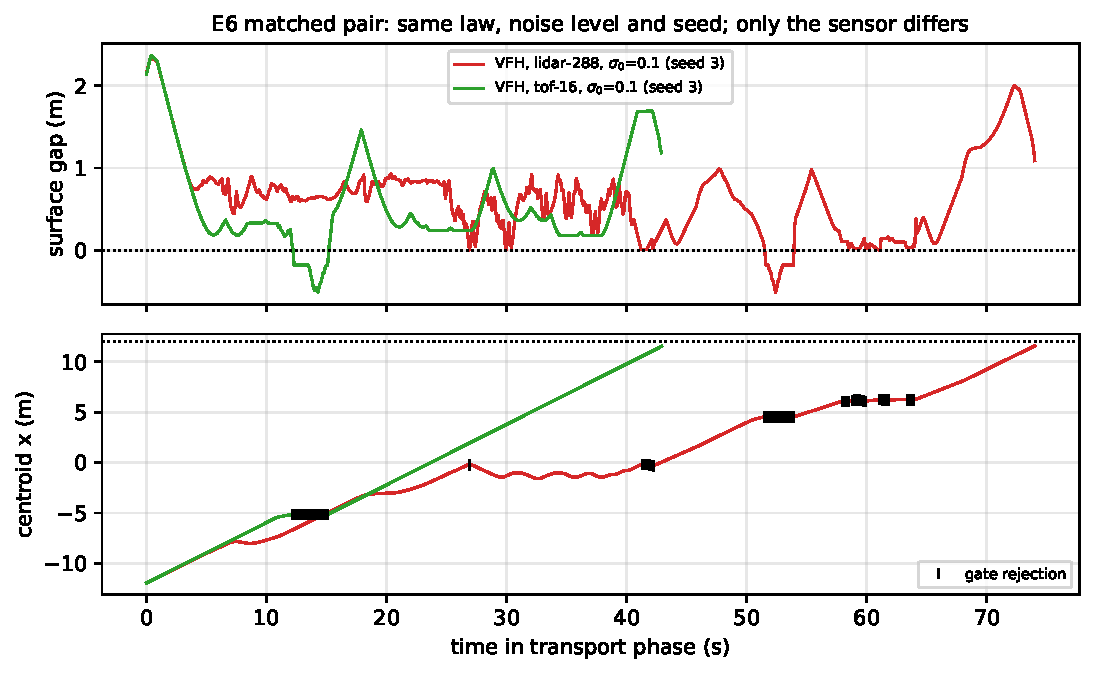
\includegraphics[width=0.85\textwidth]{figures/e6_timeseries.pdf}
\caption{E6 matched pair: deterministic VFH at the higher noise level on
lidar-288 and on tof-16, same seed (the lidar cell's worst seed by gate
rejections).}
\label{fig:e6ts}
\end{figure}

\paragraph{How to read E6.} Within an x-group the bars differ only by law;
across groups only the sensor changes. The lidar cells reuse the E2
simulations of the first ten seeds at the same $\sigma_0$ (each
configuration is run once), so they must agree with Table~\ref{tab:e2} up
to the ten extra seeds E2 carries. The two caveats of E3 apply: a narrow fan reacts to
fewer side obstacles, which can look like better behaviour, and is blind
to side and rear traffic, which shows up as mover contacts.

\subsection{E7 --- other environments}
\label{sec:e7}

The warehouse is one layout. E7 repeats the eight-law comparison at a low and
a high noise level in two further worlds with the same bounds, start and
goal: an \textbf{open plaza} (fourteen compact obstacles, no aisles,
traffic that \emph{crosses} the route) and a \textbf{serpentine maze}
(three baffles with alternating $3.25$~m gates, forcing four turns of about
$90^\circ$). In the maze every law is given the same four-waypoint global
route: a reactive law has no reason to drive away from the goal toward a
gate, so the experiment tests local steering along a given route, not
global planning.

\begin{figure}[H]
\centering
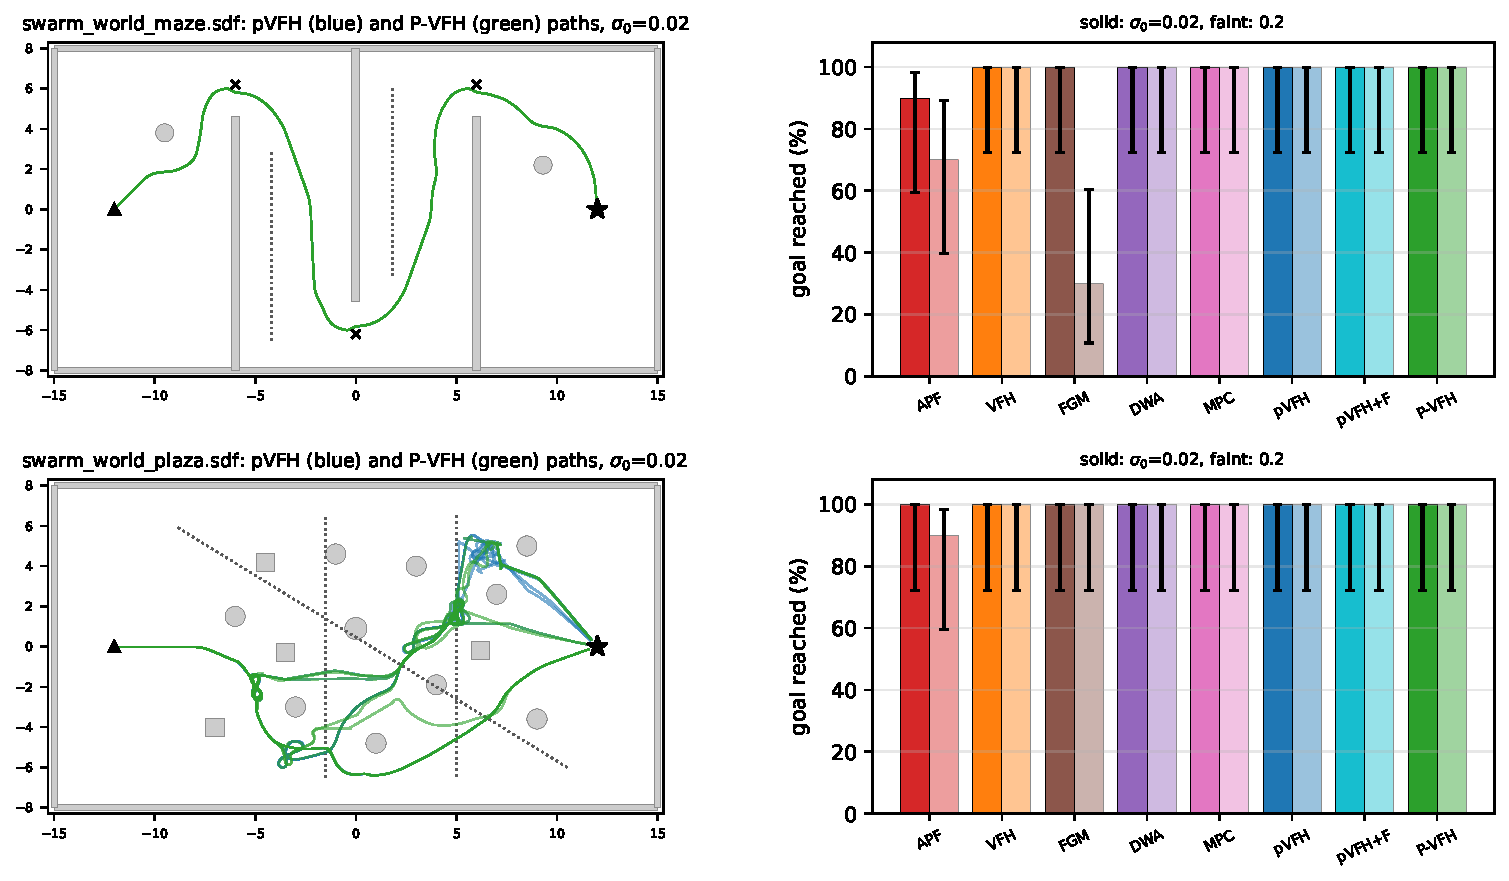
\includegraphics[width=\textwidth]{figures/e7_environments.pdf}
\caption{E7. Left: the worlds with the paths of the two horizon-equipped
histogram laws at the low noise level. Right: reach rate per law (solid:
low noise; faint: high noise).}
\label{fig:e7}
\end{figure}

% AUTO-GENERATED by matlab/make_paper_figures.py -- do not edit
\begin{table}[H]
\centering\scriptsize
\begin{tabular}{@{}lllrrrrrrr@{}}
\toprule
\textbf{World} & \textbf{$\sigma_0$} & \textbf{Law} & \textbf{Reach} [95\% CI, \%] & \textbf{Gate rej.} & \textbf{Static} & \textbf{Mover} & \textbf{Min gap (m)} [95\% CI] & \textbf{Eff.} & \textbf{Time (s)} \\
\midrule
maze & 0.02 & APF & 9/10 [60,98] & 199.8 & 0 & 0.0 & 0.04 [0.01,0.08] & 0.23 & 198 \\
maze & 0.02 & VFH & 10/10 [72,100] & 0.0 & 0 & 0.0 & 0.27 [0.27,0.27] & 0.50 & 84 \\
maze & 0.02 & FGM & 10/10 [72,100] & 12.4 & 0 & 0.0 & 0.01 [0.00,0.01] & 0.40 & 108 \\
maze & 0.02 & DWA & 10/10 [72,100] & 0.0 & 0 & 0.0 & 0.13 [0.12,0.13] & 0.51 & 83 \\
maze & 0.02 & MPC & 10/10 [72,100] & 0.0 & 0 & 0.0 & 0.28 [0.27,0.29] & 0.52 & 81 \\
maze & 0.02 & pVFH & 10/10 [72,100] & 0.0 & 0 & 0.0 & 0.27 [0.27,0.27] & 0.50 & 84 \\
maze & 0.02 & pVFH+F & 10/10 [72,100] & 0.0 & 0 & 0.0 & 0.27 [0.26,0.27] & 0.50 & 84 \\
maze & 0.02 & P-VFH & 10/10 [72,100] & 0.0 & 0 & 0.0 & 0.27 [0.26,0.27] & 0.50 & 84 \\
maze & 0.2 & APF & 7/10 [40,89] & 1341.1 & 0 & 0.0 & 0.01 [0.00,0.01] & 0.15 & 368 \\
maze & 0.2 & VFH & 10/10 [72,100] & 0.5 & 0 & 0.0 & 0.10 [0.06,0.15] & 0.40 & 105 \\
maze & 0.2 & FGM & 3/10 [11,60] & 3386.4 & 0 & 0.0 & 0.01 [0.00,0.03] & 0.15 & 534 \\
maze & 0.2 & DWA & 10/10 [72,100] & 0.0 & 0 & 0.0 & 0.33 [0.32,0.34] & 0.50 & 86 \\
maze & 0.2 & MPC & 10/10 [72,100] & 0.0 & 0 & 0.0 & 0.45 [0.43,0.47] & 0.50 & 84 \\
maze & 0.2 & pVFH & 10/10 [72,100] & 2.2 & 0 & 0.0 & 0.08 [0.04,0.12] & 0.40 & 105 \\
maze & 0.2 & pVFH+F & 10/10 [72,100] & 0.0 & 0 & 0.0 & 0.24 [0.23,0.25] & 0.50 & 84 \\
maze & 0.2 & P-VFH & 10/10 [72,100] & 0.0 & 0 & 0.0 & 0.24 [0.23,0.25] & 0.50 & 84 \\
\midrule
plaza & 0.02 & APF & 10/10 [72,100] & 85.3 & 0 & 25.5 & -0.33 [-0.47,-0.17] & 0.41 & 110 \\
plaza & 0.02 & VFH & 10/10 [72,100] & 33.2 & 0 & 18.3 & -0.17 [-0.34,-0.01] & 0.58 & 79 \\
plaza & 0.02 & FGM & 10/10 [72,100] & 63.8 & 0 & 27.5 & -0.35 [-0.50,-0.20] & 0.54 & 84 \\
plaza & 0.02 & DWA & 10/10 [72,100] & 27.0 & 0 & 14.7 & -0.01 [-0.15,0.09] & 0.74 & 65 \\
plaza & 0.02 & MPC & 10/10 [72,100] & 0.0 & 0 & 0.0 & 0.09 [0.05,0.13] & 0.88 & 50 \\
plaza & 0.02 & pVFH & 10/10 [72,100] & 44.7 & 0 & 25.9 & -0.13 [-0.32,0.06] & 0.55 & 88 \\
plaza & 0.02 & pVFH+F & 10/10 [72,100] & 36.8 & 0 & 15.2 & -0.14 [-0.32,0.04] & 0.55 & 84 \\
plaza & 0.02 & P-VFH & 10/10 [72,100] & 35.4 & 0 & 14.8 & -0.13 [-0.32,0.06] & 0.59 & 79 \\
plaza & 0.2 & APF & 9/10 [60,98] & 251.7 & 0 & 27.3 & -0.34 [-0.50,-0.16] & 0.34 & 144 \\
plaza & 0.2 & VFH & 10/10 [72,100] & 58.6 & 0 & 22.9 & -0.21 [-0.35,-0.08] & 0.54 & 84 \\
plaza & 0.2 & FGM & 10/10 [72,100] & 53.3 & 0 & 21.2 & -0.24 [-0.39,-0.10] & 0.51 & 88 \\
plaza & 0.2 & DWA & 10/10 [72,100] & 5.4 & 0 & 0.0 & 0.17 [0.09,0.25] & 0.69 & 65 \\
plaza & 0.2 & MPC & 10/10 [72,100] & 0.2 & 0 & 0.0 & 0.25 [0.12,0.38] & 0.75 & 58 \\
plaza & 0.2 & pVFH & 10/10 [72,100] & 56.9 & 0 & 16.9 & -0.22 [-0.35,-0.10] & 0.54 & 84 \\
plaza & 0.2 & pVFH+F & 10/10 [72,100] & 55.7 & 0 & 18.0 & -0.17 [-0.31,-0.05] & 0.53 & 87 \\
plaza & 0.2 & P-VFH & 10/10 [72,100] & 64.0 & 0 & 28.6 & -0.23 [-0.36,-0.09] & 0.53 & 87 \\
\bottomrule
\end{tabular}
\caption{E7, every cell. Reach: runs reaching the goal, Wilson interval. Gate rej.: mean steps per run in which the safety gate refused the commanded motion. Static: total static-contact steps over the cell (must be 0). Mover: mean steps per run in contact with a mover. Min gap: mean over runs of the per-run minimum surface gap, bootstrap interval. $\dagger$ = legacy pre-fix table, where this column is the old collision-step count.}
\label{tab:e7}
\end{table}


\paragraph{How to read E7.} The question is whether the \emph{ordering} of
the laws seen in the warehouse persists, not whether the absolute values
do. Three layouts are still a small sample of the space of environments,
and all three were designed by the authors; E7 widens the evidence, it
does not make it general.

\subsection{E8 --- traffic speed}
\label{sec:e8}

\begin{figure}[H]
\centering
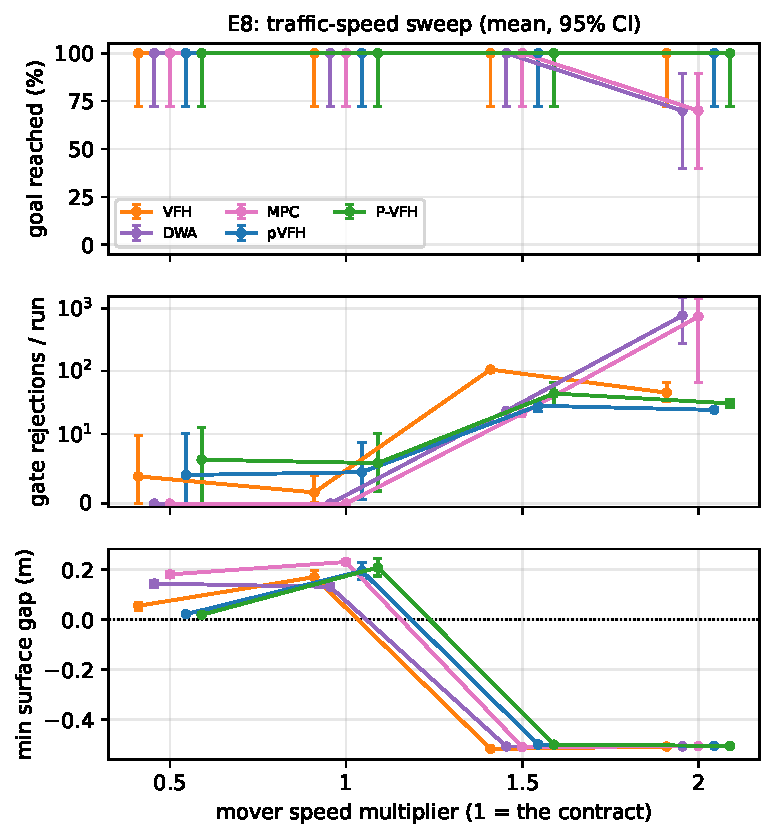
\includegraphics[width=0.74\textwidth]{figures/e8_traffic.pdf}
\caption{E8: the three metrics against the mover-speed multiplier.}
\label{fig:e8}
\end{figure}

% AUTO-GENERATED by matlab/make_paper_figures.py -- do not edit
\begin{table}[H]
\centering\scriptsize
\begin{tabular}{@{}llrrrrrrr@{}}
\toprule
\textbf{Law} & \textbf{Mover speed x} & \textbf{Reach} [95\% CI, \%] & \textbf{Gate rej.} & \textbf{Static} & \textbf{Mover} & \textbf{Min gap (m)} [95\% CI] & \textbf{Eff.} & \textbf{Time (s)} \\
\midrule
VFH & 0.5 & 10/10 [72,100] & 3.9 & 0 & 0.0 & 0.06 [0.04,0.07] & 0.88 & 50 \\
VFH & 1 & 10/10 [72,100] & 1.6 & 0 & 0.0 & 0.17 [0.14,0.20] & 0.90 & 49 \\
VFH & 1.5 & 10/10 [72,100] & 106.1 & 0 & 92.2 & -0.52 [-0.52,-0.51] & 0.90 & 61 \\
VFH & 2 & 10/10 [72,100] & 45.3 & 0 & 30.9 & -0.51 [-0.51,-0.50] & 0.81 & 59 \\
\midrule
DWA & 0.5 & 10/10 [72,100] & 0.0 & 0 & 0.0 & 0.14 [0.13,0.16] & 0.94 & 49 \\
DWA & 1 & 10/10 [72,100] & 0.0 & 0 & 0.0 & 0.13 [0.12,0.14] & 0.91 & 50 \\
DWA & 1.5 & 10/10 [72,100] & 23.3 & 0 & 19.7 & -0.51 [-0.51,-0.50] & 0.96 & 50 \\
DWA & 2 & 7/10 [40,89] & 770.4 & 0 & 35.9 & -0.51 [-0.51,-0.50] & 0.75 & 134 \\
\midrule
MPC & 0.5 & 10/10 [72,100] & 0.0 & 0 & 0.0 & 0.18 [0.17,0.19] & 0.95 & 47 \\
MPC & 1 & 10/10 [72,100] & 0.0 & 0 & 0.0 & 0.23 [0.22,0.24] & 0.97 & 46 \\
MPC & 1.5 & 10/10 [72,100] & 21.3 & 0 & 19.7 & -0.51 [-0.51,-0.51] & 0.98 & 48 \\
MPC & 2 & 7/10 [40,89] & 740.7 & 0 & 35.6 & -0.51 [-0.51,-0.50] & 0.68 & 133 \\
\midrule
pVFH & 0.5 & 10/10 [72,100] & 4.1 & 0 & 0.0 & 0.02 [0.02,0.03] & 0.88 & 50 \\
pVFH & 1 & 10/10 [72,100] & 4.5 & 0 & 0.0 & 0.19 [0.16,0.23] & 0.89 & 50 \\
pVFH & 1.5 & 10/10 [72,100] & 28.1 & 0 & 20.0 & -0.50 [-0.51,-0.49] & 0.68 & 66 \\
pVFH & 2 & 10/10 [72,100] & 24.1 & 0 & 15.7 & -0.50 [-0.51,-0.50] & 0.80 & 58 \\
\midrule
P-VFH & 0.5 & 10/10 [72,100] & 6.3 & 0 & 0.0 & 0.02 [0.01,0.03] & 0.88 & 51 \\
P-VFH & 1 & 10/10 [72,100] & 5.8 & 0 & 0.0 & 0.21 [0.17,0.24] & 0.89 & 50 \\
P-VFH & 1.5 & 10/10 [72,100] & 44.0 & 0 & 25.3 & -0.50 [-0.50,-0.50] & 0.70 & 66 \\
P-VFH & 2 & 10/10 [72,100] & 30.6 & 0 & 19.2 & -0.50 [-0.51,-0.50] & 0.81 & 58 \\
\bottomrule
\end{tabular}
\caption{E8. Reach: runs reaching the goal, Wilson interval. Gate rej.: mean steps per run in which the safety gate refused the commanded motion. Static: total static-contact steps over the cell (must be 0). Mover: mean steps per run in contact with a mover. Min gap: mean over runs of the per-run minimum surface gap, bootstrap interval. $\dagger$ = legacy pre-fix table, where this column is the old collision-step count.}
\label{tab:e8}
\end{table}


\paragraph{How to read E8.} The multiplier scales every mover's contracted
speed (at $2\times$ the fastest mover does $1.8$~m/s, three times the
formation's speed). The two laws without a prediction horizon
(\code{vfh}, \code{dwa}) see a mover only where it is now; the two with
one see where it will be over the next $0.5$~s. The horizon is fixed, so a
faster mover covers more ground inside it: expect the horizon to matter
more as speed rises, and expect every law to accumulate mover contacts
eventually, since the movers never yield.

\subsection{E9 --- ablation of the anti-deadlock layer}
\label{sec:e9}

\begin{figure}[H]
\centering
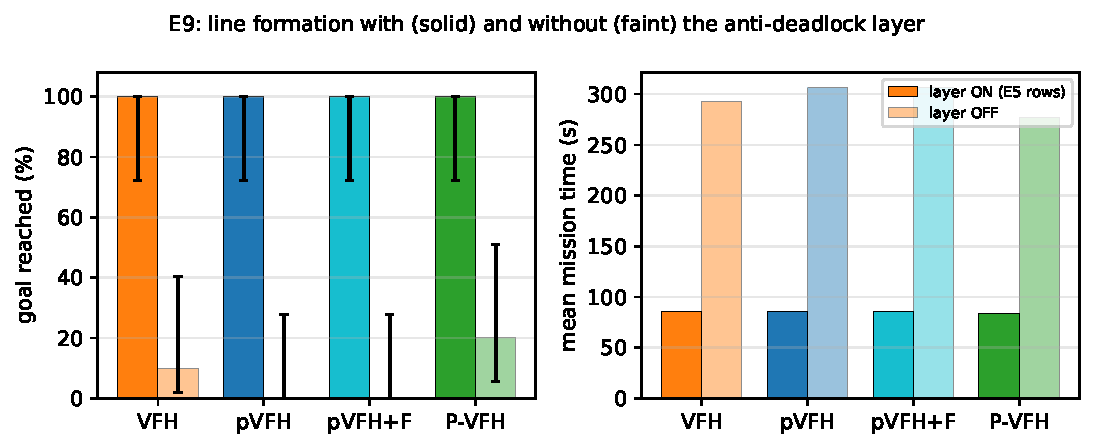
\includegraphics[width=0.8\textwidth]{figures/e9_adl.pdf}
\caption{E9: line formation with and without the anti-deadlock layer.}
\label{fig:e9}
\end{figure}

% AUTO-GENERATED by matlab/make_paper_figures.py -- do not edit
\begin{table}[H]
\centering\scriptsize
\begin{tabular}{@{}llrrrrrrr@{}}
\toprule
\textbf{Law} & \textbf{Layer} & \textbf{Reach} [95\% CI, \%] & \textbf{Gate rej.} & \textbf{Static} & \textbf{Mover} & \textbf{Min gap (m)} [95\% CI] & \textbf{Eff.} & \textbf{Time (s)} \\
\midrule
VFH & ON & 10/10 [72,100] & 13.0 & 0 & 4.1 & -0.08 [-0.22,0.02] & 0.51 & 85 \\
VFH & OFF & 1/10 [2,40] & 19.1 & 0 & 7.0 & -0.10 [-0.16,-0.03] & 0.08 & 293 \\
pVFH & ON & 10/10 [72,100] & 10.8 & 0 & 2.1 & -0.01 [-0.13,0.08] & 0.50 & 86 \\
pVFH & OFF & 0/10 [0,28] & 12.0 & 0 & 0.4 & -0.00 [-0.04,0.02] & 0.06 & 306 \\
pVFH+F & ON & 10/10 [72,100] & 9.8 & 0 & 0.1 & 0.01 [-0.04,0.05] & 0.50 & 86 \\
pVFH+F & OFF & 0/10 [0,28] & 12.9 & 0 & 0.0 & 0.01 [0.01,0.03] & 0.06 & 306 \\
P-VFH & ON & 10/10 [72,100] & 10.7 & 0 & 1.8 & -0.02 [-0.11,0.03] & 0.52 & 84 \\
P-VFH & OFF & 2/10 [6,51] & 15.5 & 0 & 0.0 & 0.01 [0.01,0.01] & 0.10 & 277 \\
\bottomrule
\end{tabular}
\caption{E9. Reach: runs reaching the goal, Wilson interval. Gate rej.: mean steps per run in which the safety gate refused the commanded motion. Static: total static-contact steps over the cell (must be 0). Mover: mean steps per run in contact with a mover. Min gap: mean over runs of the per-run minimum surface gap, bootstrap interval. $\dagger$ = legacy pre-fix table, where this column is the old collision-step count.}
\label{tab:e9}
\end{table}


\paragraph{How to read E9.} The layer belongs to the mission, not to any
steering law, and every law gets it. This ablation shows how much of the
line-formation result is owed to it: if a law reaches the goal only with
the layer on, the credit for that cell belongs to the layer.

\subsection{E10 --- localisation error}
\label{sec:e10}

Every other experiment gives the controller its true pose. Here the
controller believes it is at the true position plus
$\mathcal{N}(0, \sigma_p^2 I)$ with a heading error of standard deviation
$20^\circ$ per metre of $\sigma_p$, redrawn every step. The scan is
physical --- taken at the true pose in the body frame --- so what the error
corrupts is the believed direction of the goal. Arrival and the safety
gate use the true pose.

\begin{figure}[H]
\centering
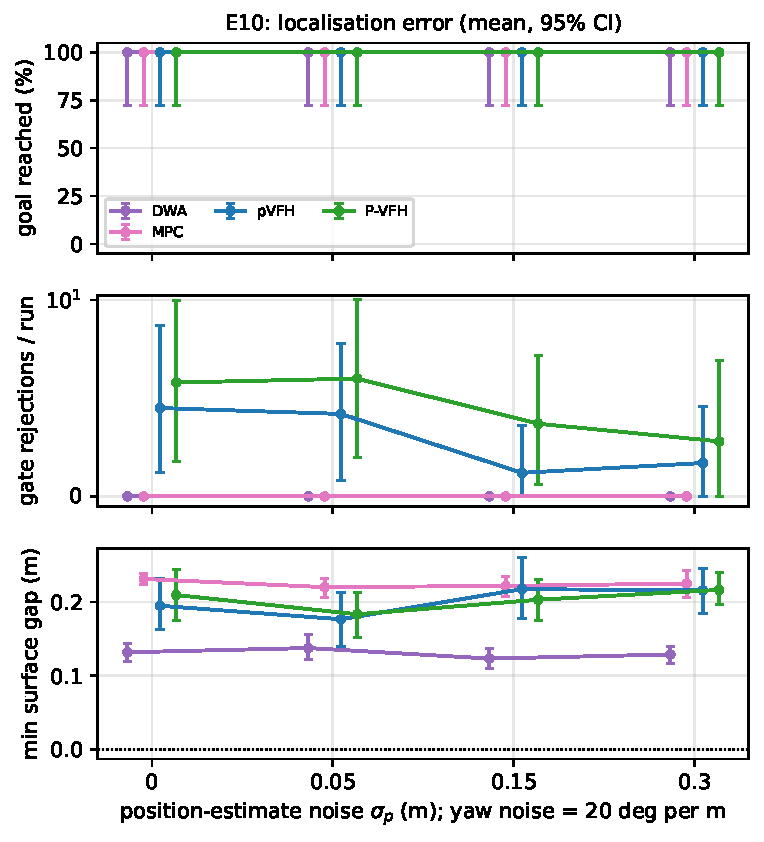
\includegraphics[width=0.74\textwidth]{figures/e10_localisation.pdf}
\caption{E10: the three metrics against the position-estimate noise.}
\label{fig:e10}
\end{figure}

% AUTO-GENERATED by matlab/make_paper_figures.py -- do not edit
\begin{table}[H]
\centering\scriptsize
\begin{tabular}{@{}llrrrrrrr@{}}
\toprule
\textbf{Law} & \textbf{Pose noise (m)} & \textbf{Reach} [95\% CI, \%] & \textbf{Gate rej.} & \textbf{Static} & \textbf{Mover} & \textbf{Min gap (m)} [95\% CI] & \textbf{Eff.} & \textbf{Time (s)} \\
\midrule
DWA & 0 & 10/10 [72,100] & 0.0 & 0 & 0.0 & 0.13 [0.12,0.14] & 0.91 & 50 \\
DWA & 0.05 & 10/10 [72,100] & 0.0 & 0 & 0.0 & 0.14 [0.12,0.16] & 0.91 & 50 \\
DWA & 0.15 & 10/10 [72,100] & 0.0 & 0 & 0.0 & 0.12 [0.11,0.14] & 0.88 & 52 \\
DWA & 0.3 & 10/10 [72,100] & 0.0 & 0 & 0.0 & 0.13 [0.12,0.14] & 0.86 & 52 \\
\midrule
MPC & 0 & 10/10 [72,100] & 0.0 & 0 & 0.0 & 0.23 [0.22,0.24] & 0.97 & 46 \\
MPC & 0.05 & 10/10 [72,100] & 0.0 & 0 & 0.0 & 0.22 [0.21,0.23] & 0.97 & 46 \\
MPC & 0.15 & 10/10 [72,100] & 0.0 & 0 & 0.0 & 0.22 [0.21,0.23] & 0.97 & 46 \\
MPC & 0.3 & 10/10 [72,100] & 0.0 & 0 & 0.0 & 0.23 [0.21,0.24] & 0.97 & 46 \\
\midrule
pVFH & 0 & 10/10 [72,100] & 4.5 & 0 & 0.0 & 0.19 [0.16,0.23] & 0.89 & 50 \\
pVFH & 0.05 & 10/10 [72,100] & 4.2 & 0 & 0.0 & 0.18 [0.14,0.21] & 0.89 & 50 \\
pVFH & 0.15 & 10/10 [72,100] & 1.2 & 0 & 0.0 & 0.22 [0.18,0.26] & 0.89 & 50 \\
pVFH & 0.3 & 10/10 [72,100] & 1.7 & 0 & 0.0 & 0.22 [0.19,0.24] & 0.88 & 50 \\
\midrule
P-VFH & 0 & 10/10 [72,100] & 5.8 & 0 & 0.0 & 0.21 [0.17,0.24] & 0.89 & 50 \\
P-VFH & 0.05 & 10/10 [72,100] & 6.0 & 0 & 0.0 & 0.18 [0.15,0.21] & 0.88 & 50 \\
P-VFH & 0.15 & 10/10 [72,100] & 3.7 & 0 & 0.0 & 0.20 [0.17,0.23] & 0.89 & 50 \\
P-VFH & 0.3 & 10/10 [72,100] & 2.8 & 0 & 0.0 & 0.22 [0.20,0.24] & 0.88 & 50 \\
\bottomrule
\end{tabular}
\caption{E10. Reach: runs reaching the goal, Wilson interval. Gate rej.: mean steps per run in which the safety gate refused the commanded motion. Static: total static-contact steps over the cell (must be 0). Mover: mean steps per run in contact with a mover. Min gap: mean over runs of the per-run minimum surface gap, bootstrap interval. $\dagger$ = legacy pre-fix table, where this column is the old collision-step count.}
\label{tab:e10}
\end{table}


\paragraph{How to read E10.} The error is white (independent each step),
which is the mild case: the heading low-pass averages much of it away. A
real localiser drifts, and a slowly varying bias is not tested here. Read
the result as an upper bound on tolerance, not as a claim of robustness to
localisation failure.

\subsection{E11 --- traffic density}
\label{sec:e11}

The warehouse contract is extended to six movers (the original three plus
three crossing ones); the experiment uses the first $N$.

\begin{figure}[H]
\centering
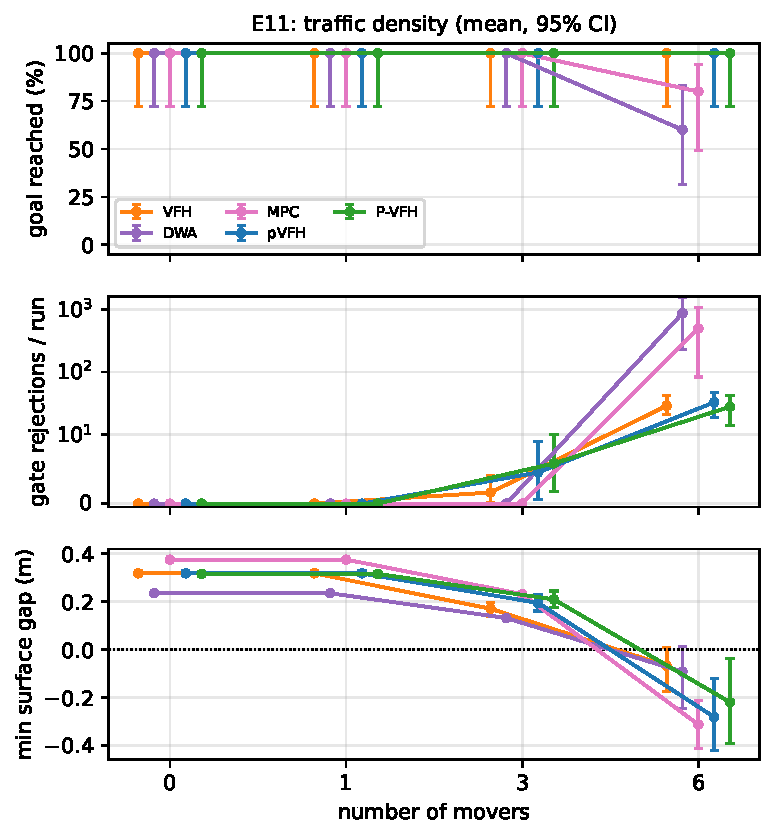
\includegraphics[width=0.74\textwidth]{figures/e11_density.pdf}
\caption{E11: the three metrics against the number of movers.}
\label{fig:e11}
\end{figure}

% AUTO-GENERATED by matlab/make_paper_figures.py -- do not edit
\begin{table}[H]
\centering\scriptsize
\begin{tabular}{@{}llrrrrrrr@{}}
\toprule
\textbf{Law} & \textbf{Movers} & \textbf{Reach} [95\% CI, \%] & \textbf{Gate rej.} & \textbf{Static} & \textbf{Mover} & \textbf{Min gap (m)} [95\% CI] & \textbf{Eff.} & \textbf{Time (s)} \\
\midrule
VFH & 0 & 10/10 [72,100] & 0.0 & 0 & 0.0 & 0.32 [0.31,0.33] & 0.95 & 47 \\
VFH & 1 & 10/10 [72,100] & 0.0 & 0 & 0.0 & 0.32 [0.31,0.33] & 0.95 & 47 \\
VFH & 3 & 10/10 [72,100] & 1.6 & 0 & 0.0 & 0.17 [0.14,0.20] & 0.90 & 49 \\
VFH & 6 & 10/10 [72,100] & 28.8 & 0 & 6.7 & -0.07 [-0.18,0.01] & 0.76 & 60 \\
\midrule
DWA & 0 & 10/10 [72,100] & 0.0 & 0 & 0.0 & 0.24 [0.23,0.24] & 0.99 & 46 \\
DWA & 1 & 10/10 [72,100] & 0.0 & 0 & 0.0 & 0.24 [0.23,0.24] & 0.98 & 47 \\
DWA & 3 & 10/10 [72,100] & 0.0 & 0 & 0.0 & 0.13 [0.12,0.14] & 0.91 & 50 \\
DWA & 6 & 6/10 [31,83] & 883.5 & 0 & 11.0 & -0.09 [-0.24,0.01] & 0.55 & 163 \\
\midrule
MPC & 0 & 10/10 [72,100] & 0.0 & 0 & 0.0 & 0.38 [0.37,0.38] & 0.99 & 45 \\
MPC & 1 & 10/10 [72,100] & 0.0 & 0 & 0.0 & 0.38 [0.37,0.38] & 0.99 & 45 \\
MPC & 3 & 10/10 [72,100] & 0.0 & 0 & 0.0 & 0.23 [0.22,0.24] & 0.97 & 46 \\
MPC & 6 & 8/10 [49,94] & 501.6 & 0 & 75.7 & -0.31 [-0.41,-0.21] & 0.64 & 116 \\
\midrule
pVFH & 0 & 10/10 [72,100] & 0.0 & 0 & 0.0 & 0.32 [0.31,0.33] & 0.95 & 47 \\
pVFH & 1 & 10/10 [72,100] & 0.0 & 0 & 0.0 & 0.32 [0.31,0.33] & 0.95 & 47 \\
pVFH & 3 & 10/10 [72,100] & 4.5 & 0 & 0.0 & 0.19 [0.16,0.23] & 0.89 & 50 \\
pVFH & 6 & 10/10 [72,100] & 32.7 & 0 & 16.1 & -0.28 [-0.42,-0.13] & 0.77 & 61 \\
\midrule
P-VFH & 0 & 10/10 [72,100] & 0.0 & 0 & 0.0 & 0.32 [0.31,0.33] & 0.95 & 47 \\
P-VFH & 1 & 10/10 [72,100] & 0.0 & 0 & 0.0 & 0.32 [0.31,0.33] & 0.95 & 47 \\
P-VFH & 3 & 10/10 [72,100] & 5.8 & 0 & 0.0 & 0.21 [0.17,0.24] & 0.89 & 50 \\
P-VFH & 6 & 10/10 [72,100] & 27.8 & 0 & 13.4 & -0.22 [-0.39,-0.04] & 0.76 & 61 \\
\bottomrule
\end{tabular}
\caption{E11. Reach: runs reaching the goal, Wilson interval. Gate rej.: mean steps per run in which the safety gate refused the commanded motion. Static: total static-contact steps over the cell (must be 0). Mover: mean steps per run in contact with a mover. Min gap: mean over runs of the per-run minimum surface gap, bootstrap interval. $\dagger$ = legacy pre-fix table, where this column is the old collision-step count.}
\label{tab:e11}
\end{table}


\paragraph{How to read E11.} The $N = 0$ column is the static-world
reference for every law; whatever a law loses between $N = 0$ and $N = 6$
is the cost of traffic. With six movers in a 30~m $\times$ 16~m hall the
movers, which never yield, will sometimes box the formation in; mover
contacts at high density say as much about the traffic model as about the
steering.

\subsection{E12 --- command-update loss}
\label{sec:e12}

With the given probability a step's steering update is lost and the
previous heading and speed command is held. This is the only
communication fault the model can express: the formation is a rigid
virtual frame, so there are no robot-to-robot messages to drop.

\begin{figure}[H]
\centering
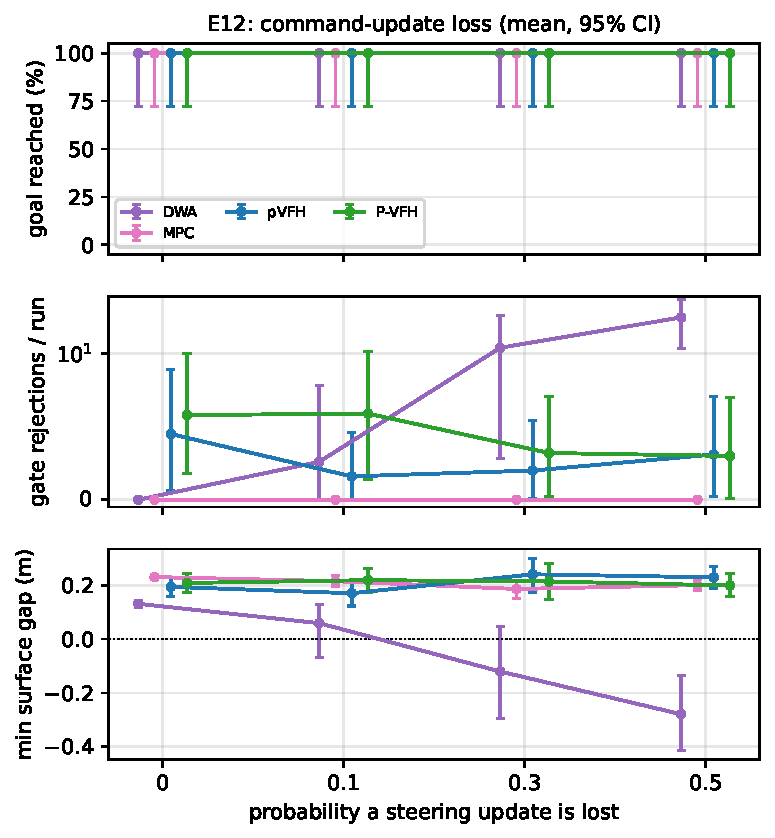
\includegraphics[width=0.74\textwidth]{figures/e12_commloss.pdf}
\caption{E12: the three metrics against the loss probability.}
\label{fig:e12}
\end{figure}

% AUTO-GENERATED by matlab/make_paper_figures.py -- do not edit
\begin{table}[H]
\centering\scriptsize
\begin{tabular}{@{}llrrrrrrr@{}}
\toprule
\textbf{Law} & \textbf{Drop prob.} & \textbf{Reach} [95\% CI, \%] & \textbf{Gate rej.} & \textbf{Static} & \textbf{Mover} & \textbf{Min gap (m)} [95\% CI] & \textbf{Eff.} & \textbf{Time (s)} \\
\midrule
DWA & 0 & 10/10 [72,100] & 0.0 & 0 & 0.0 & 0.13 [0.12,0.14] & 0.91 & 50 \\
DWA & 0.1 & 10/10 [72,100] & 2.6 & 0 & 2.5 & 0.06 [-0.07,0.13] & 0.91 & 51 \\
DWA & 0.3 & 10/10 [72,100] & 11.1 & 0 & 9.9 & -0.12 [-0.30,0.05] & 0.90 & 52 \\
DWA & 0.5 & 10/10 [72,100] & 18.9 & 0 & 16.4 & -0.28 [-0.41,-0.13] & 0.90 & 53 \\
\midrule
MPC & 0 & 10/10 [72,100] & 0.0 & 0 & 0.0 & 0.23 [0.22,0.24] & 0.97 & 46 \\
MPC & 0.1 & 10/10 [72,100] & 0.0 & 0 & 0.0 & 0.22 [0.19,0.24] & 0.97 & 46 \\
MPC & 0.3 & 10/10 [72,100] & 0.0 & 0 & 0.0 & 0.19 [0.15,0.22] & 0.96 & 46 \\
MPC & 0.5 & 10/10 [72,100] & 0.0 & 0 & 0.0 & 0.20 [0.18,0.22] & 0.96 & 46 \\
\midrule
pVFH & 0 & 10/10 [72,100] & 4.5 & 0 & 0.0 & 0.19 [0.16,0.23] & 0.89 & 50 \\
pVFH & 0.1 & 10/10 [72,100] & 1.6 & 0 & 0.0 & 0.17 [0.13,0.22] & 0.88 & 50 \\
pVFH & 0.3 & 10/10 [72,100] & 2.0 & 0 & 0.0 & 0.24 [0.18,0.30] & 0.87 & 51 \\
pVFH & 0.5 & 10/10 [72,100] & 3.1 & 0 & 0.0 & 0.23 [0.19,0.27] & 0.87 & 51 \\
\midrule
P-VFH & 0 & 10/10 [72,100] & 5.8 & 0 & 0.0 & 0.21 [0.17,0.24] & 0.89 & 50 \\
P-VFH & 0.1 & 10/10 [72,100] & 5.9 & 0 & 0.0 & 0.22 [0.18,0.26] & 0.89 & 50 \\
P-VFH & 0.3 & 10/10 [72,100] & 3.2 & 0 & 0.0 & 0.21 [0.14,0.28] & 0.87 & 51 \\
P-VFH & 0.5 & 10/10 [72,100] & 3.0 & 0 & 0.0 & 0.20 [0.16,0.24] & 0.87 & 51 \\
\bottomrule
\end{tabular}
\caption{E12. Reach: runs reaching the goal, Wilson interval. Gate rej.: mean steps per run in which the safety gate refused the commanded motion. Static: total static-contact steps over the cell (must be 0). Mover: mean steps per run in contact with a mover. Min gap: mean over runs of the per-run minimum surface gap, bootstrap interval. $\dagger$ = legacy pre-fix table, where this column is the old collision-step count.}
\label{tab:e12}
\end{table}


\paragraph{How to read E12.} Losses are independent per step, so even at
$0.5$ the expected gap between updates is two steps ($0.2$~s). Burst
losses, delays and per-robot faults are outside what this experiment
covers.

\subsection{E13 --- randomised layouts}
\label{sec:e13}

The three worlds so far were designed by hand. E13 uses ten layouts
produced by a seeded generator (\code{make\_random\_worlds.py}): 12--18
posts and crates placed uniformly at random on the same floor, accepted
only if the start and goal are clear, the corridor bottleneck is at least
$1.30$~m and the straight start--goal line is blocked; two crossing movers
per layout. The layouts were generated once, before any result existed,
and are not regenerated.

\begin{figure}[H]
\centering
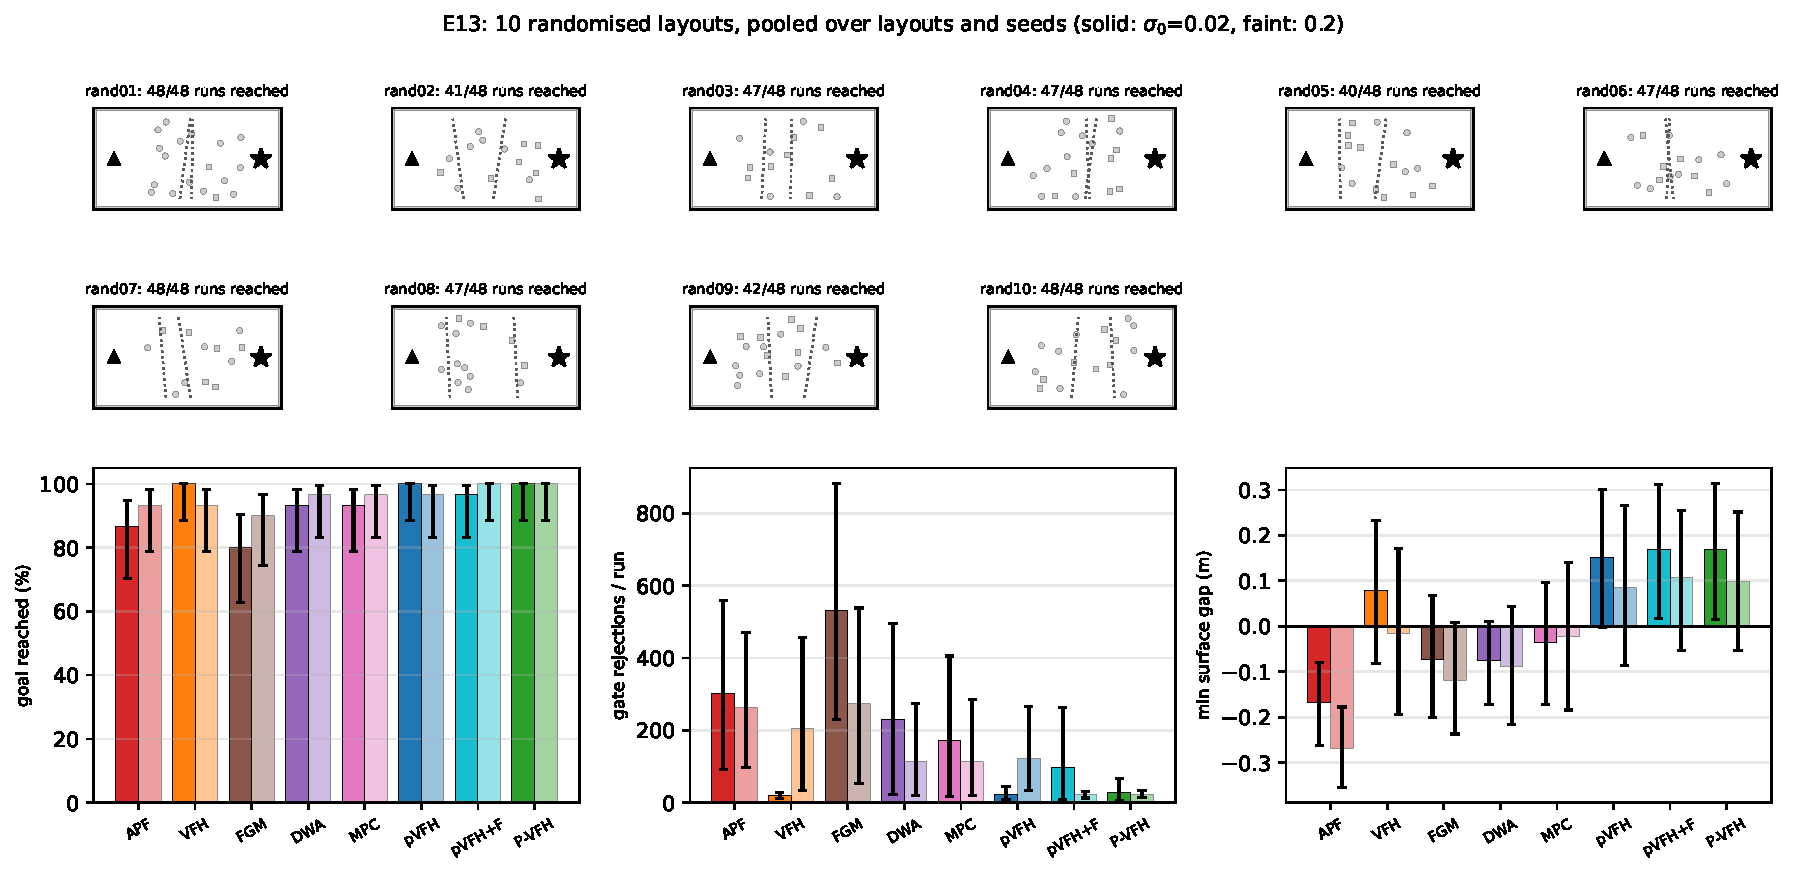
\includegraphics[width=\textwidth]{figures/e13_random.pdf}
\caption{E13. Top: the ten layouts with the number of runs (all laws, both
noise levels) that reached the goal. Bottom: reach, gate rejections and
gap per law, pooled over layouts and seeds (solid: low noise; faint: high
noise).}
\label{fig:e13}
\end{figure}

% AUTO-GENERATED by matlab/make_paper_figures.py -- do not edit
\begin{table}[H]
\centering\scriptsize
\begin{tabular}{@{}llrrrrrrr@{}}
\toprule
\textbf{$\sigma_0$} & \textbf{Law} & \textbf{Reach} [95\% CI, \%] & \textbf{Gate rej.} & \textbf{Static} & \textbf{Mover} & \textbf{Min gap (m)} [95\% CI] & \textbf{Eff.} & \textbf{Time (s)} \\
\midrule
0.02 & APF & 26/30 [70,95] & 302.5 & 0 & 22.3 & -0.17 [-0.26,-0.08] & 0.48 & 115 \\
0.02 & VFH & 30/30 [89,100] & 19.4 & 0 & 12.0 & 0.08 [-0.08,0.24] & 0.81 & 58 \\
0.02 & FGM & 24/30 [63,90] & 532.2 & 0 & 29.4 & -0.07 [-0.20,0.06] & 0.64 & 119 \\
0.02 & DWA & 28/30 [79,98] & 231.1 & 0 & 51.2 & -0.08 [-0.17,0.01] & 0.76 & 80 \\
0.02 & MPC & 28/30 [79,98] & 172.7 & 0 & 32.9 & -0.04 [-0.17,0.10] & 0.81 & 72 \\
0.02 & pVFH & 30/30 [89,100] & 22.5 & 0 & 10.4 & 0.15 [-0.01,0.30] & 0.76 & 61 \\
0.02 & pVFH+F & 29/30 [83,99] & 95.8 & 0 & 15.1 & 0.17 [0.02,0.31] & 0.75 & 68 \\
0.02 & P-VFH & 30/30 [89,100] & 29.2 & 0 & 11.3 & 0.17 [0.01,0.31] & 0.76 & 63 \\
\midrule
0.2 & APF & 28/30 [79,98] & 261.8 & 0 & 23.1 & -0.27 [-0.36,-0.18] & 0.44 & 122 \\
0.2 & VFH & 28/30 [79,98] & 205.4 & 0 & 26.2 & -0.02 [-0.19,0.17] & 0.71 & 84 \\
0.2 & FGM & 27/30 [74,97] & 272.7 & 0 & 16.8 & -0.12 [-0.24,0.01] & 0.58 & 100 \\
0.2 & DWA & 29/30 [83,99] & 114.0 & 0 & 19.7 & -0.09 [-0.22,0.04] & 0.77 & 71 \\
0.2 & MPC & 29/30 [83,99] & 113.0 & 0 & 25.6 & -0.02 [-0.19,0.14] & 0.81 & 66 \\
0.2 & pVFH & 29/30 [83,99] & 122.5 & 0 & 12.9 & 0.08 [-0.09,0.26] & 0.68 & 81 \\
0.2 & pVFH+F & 30/30 [89,100] & 21.5 & 0 & 9.0 & 0.11 [-0.04,0.26] & 0.74 & 64 \\
0.2 & P-VFH & 30/30 [89,100] & 23.1 & 0 & 8.9 & 0.10 [-0.05,0.25] & 0.74 & 64 \\
\bottomrule
\end{tabular}
\caption{E13. Reach: runs reaching the goal, Wilson interval. Gate rej.: mean steps per run in which the safety gate refused the commanded motion. Static: total static-contact steps over the cell (must be 0). Mover: mean steps per run in contact with a mover. Min gap: mean over runs of the per-run minimum surface gap, bootstrap interval. $\dagger$ = legacy pre-fix table, where this column is the old collision-step count.}
\label{tab:e13}
\end{table}


\paragraph{How to read E13.} The intervals pool 30 runs per cell, but those
runs come from only ten layouts, so they are not 30 independent samples of
``environments''; the paired tests in Table~\ref{tab:stats} pair on
(layout, seed). A layout on which every law fails says something about the
layout; a law that fails where others succeed says something about the law
--- the per-layout counts in the top panel separate the two. The layouts
are all of one type (sparse convex obstacles on an open floor); corridors
and concave traps are represented only by the warehouse and the maze.

\subsection{E14 --- load-feasible motion}
\label{sec:e14}

Everywhere else the rigid frame may turn at up to $3$~rad/s, which asks the
outer robot for speeds far above the centre's $0.6$~m/s (the peak is
reported for every run as \code{max\_robot\_speed}). E14 switches on the
motion limits of \S\ref{sec:gate} --- outer-robot speed
$\le 1.0$~m/s, bounded yaw acceleration and lateral acceleration --- and
repeats the E1 missions.

\begin{figure}[H]
\centering
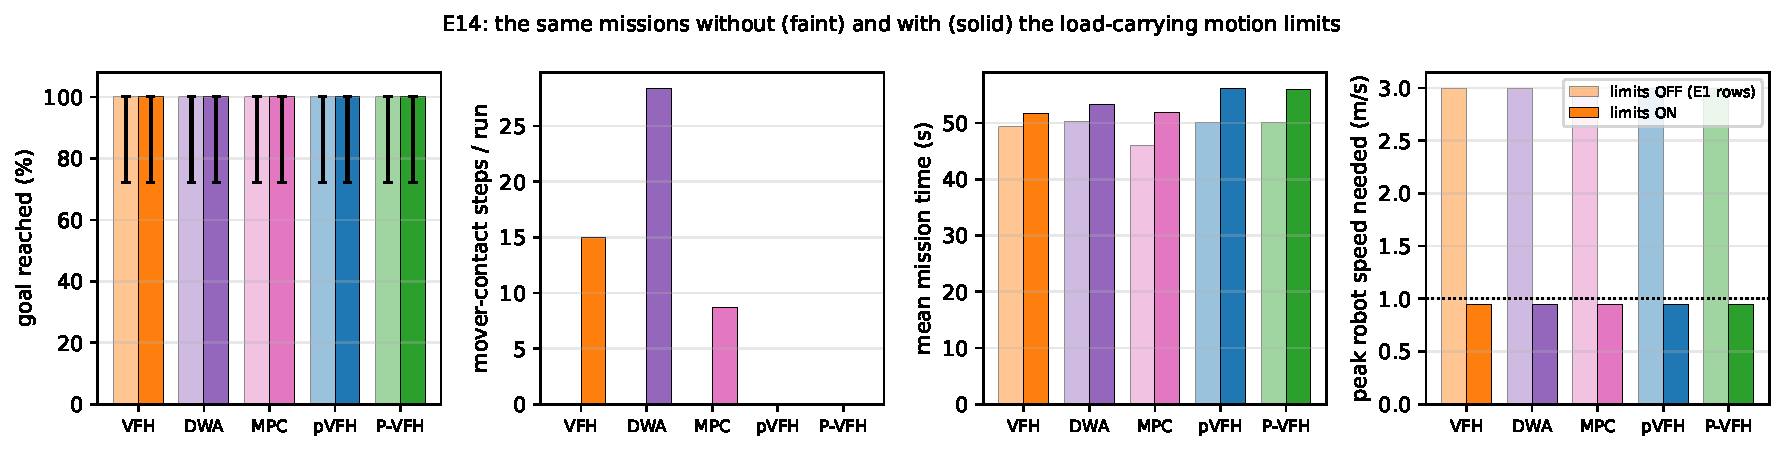
\includegraphics[width=\textwidth]{figures/e14_limits.pdf}
\caption{E14: reach rate, mover-contact steps, mission time and the peak
robot speed the motion required, without and with the limits (dotted line:
the $1.0$~m/s limit).}
\label{fig:e14}
\end{figure}

% AUTO-GENERATED by matlab/make_paper_figures.py -- do not edit
\begin{table}[H]
\centering\scriptsize
\begin{tabular}{@{}llrrrrrrr@{}}
\toprule
\textbf{Law} & \textbf{Limits} & \textbf{Reach} [95\% CI, \%] & \textbf{Gate rej.} & \textbf{Static} & \textbf{Mover} & \textbf{Min gap (m)} [95\% CI] & \textbf{Eff.} & \textbf{Time (s)} \\
\midrule
VFH & OFF & 10/10 [72,100] & 1.6 & 0 & 0.0 & 0.17 [0.14,0.20] & 0.90 & 49 \\
VFH & ON & 10/10 [72,100] & 16.7 & 0 & 15.0 & -0.19 [-0.20,-0.18] & 0.93 & 52 \\
DWA & OFF & 10/10 [72,100] & 0.0 & 0 & 0.0 & 0.13 [0.12,0.14] & 0.91 & 50 \\
DWA & ON & 10/10 [72,100] & 29.4 & 0 & 28.4 & -0.49 [-0.50,-0.49] & 0.97 & 53 \\
MPC & OFF & 10/10 [72,100] & 0.0 & 0 & 0.0 & 0.23 [0.22,0.24] & 0.97 & 46 \\
MPC & ON & 10/10 [72,100] & 15.3 & 0 & 8.7 & -0.07 [-0.14,-0.00] & 0.92 & 52 \\
pVFH & OFF & 10/10 [72,100] & 4.5 & 0 & 0.0 & 0.19 [0.16,0.23] & 0.89 & 50 \\
pVFH & ON & 10/10 [72,100] & 23.9 & 0 & 0.0 & 0.08 [0.06,0.09] & 0.88 & 56 \\
P-VFH & OFF & 10/10 [72,100] & 5.8 & 0 & 0.0 & 0.21 [0.17,0.24] & 0.89 & 50 \\
P-VFH & ON & 10/10 [72,100] & 21.4 & 0 & 0.0 & 0.08 [0.06,0.10] & 0.88 & 56 \\
\bottomrule
\end{tabular}
\caption{E14. Reach: runs reaching the goal, Wilson interval. Gate rej.: mean steps per run in which the safety gate refused the commanded motion. Static: total static-contact steps over the cell (must be 0). Mover: mean steps per run in contact with a mover. Min gap: mean over runs of the per-run minimum surface gap, bootstrap interval. $\dagger$ = legacy pre-fix table, where this column is the old collision-step count.}
\label{tab:e14}
\end{table}


\paragraph{How to read E14.} This experiment measures a weakness of the
whole study rather than a strength of any law. The steering parameters
(the $0.5$~s prediction horizon, the slow-down-near-movers rule) were
tuned for an agile body; with the limits on the formation is slower
through the chicanes and can still be in an aisle when traffic arrives. Table~\ref{tab:e14} shows exactly that for P-VFH and \code{vfh}. Read the limits-off columns of
every other experiment with the rightmost panel in mind: where the peak
robot speed is far above $1$~m/s, the trajectories shown are not ones real
robots under a load could follow, and making them so is a re-tuning task
that this report does not carry out.

\subsection{Findings (third grid of 2 October 2026, 2\,730 runs)}
\label{sec:findings}

This subsection is written by hand from the tables above and is tied to
that grid: the one run on the final code (kernel defect fixed, range
filter added, stall detector at $15$~s). Two earlier grids are archived
and their findings withdrawn. No run had a static-contact step.

\paragraph{1. The range filter removes most of the noise sensitivity of
the histogram in the warehouse (E2).} The step \code{pvfh} $\to$
\code{pvfh\_filt} changes nothing at $\sigma_0 = 0.02$~m ($50$~s, three
rejections per run either way) and a great deal above it. At
$\sigma_0 = 0.10$: mission time $77 \to 53$~s, gate rejections
$39 \to 2$, mover-contact steps $22 \to 0$, minimum gap $-0.26 \to
+0.16$~m. At $0.20$: $89 \to 62$~s, rejections $46 \to 11$, mover contact
$18 \to 5$. At $0.40$: $125 \to 84$~s, rejections $180 \to 38$. Paired by
seed, P-VFH against \code{pvfh} gains $+0.41$~m of minimum gap at
$\sigma_0 = 0.10$ and $+0.34$~m at $0.20$, with intervals excluding zero
(Table~\ref{tab:stats}). The filter has a limit: at $0.40$~m the filtered
laws are also in contact with a mover for about $19$ steps per run and
the gap difference from \code{pvfh} is no longer resolved.

\paragraph{2. The expected kernel is not shown to add anything (E2, E7,
E13).} P-VFH against \code{pvfh\_filt} --- the same filter, deterministic
versus expected kernel --- differs by a few hundredths of a metre in gap
and a handful of rejections, and every interval includes zero, at every
noise level in the warehouse and likewise in the maze, the plaza and the
random layouts. The open question of \S\ref{sec:e2} is answered in the
negative: the probabilistic occupancy is not what produces the
robustness; the noise-model-driven filter is. \S\ref{sec:pvfh} gives the
structural reason.

\paragraph{3. The filter also helps in the maze and on the random
layouts at high noise; on the plaza nothing helps (E7, E13).} In the maze
at $\sigma_0 = 0.20$ both filtered laws finish in $84$~s with no
rejections where \code{vfh} and \code{pvfh} take $105$~s. On the ten
random layouts at $\sigma_0 = 0.20$ the filtered laws take $64$~s with
about $22$ rejections per run against $81$--$84$~s and $120$--$205$
rejections unfiltered. On the plaza all four histogram laws take
$79$--$88$~s and are in contact with crossing movers for $15$--$29$ steps
per run, filtered or not, while the MPC baseline takes $50$--$58$~s with
no contact and no rejections.

\paragraph{4. Against the external baselines the picture depends on the
environment and the traffic (E1, E7, E8, E11, E13).} At the contracted
traffic in the warehouse the MPC baseline is the fastest law ($46$~s)
with no rejections and no contact, and it is clearly the best on the
plaza. On the random layouts the histogram laws are as fast or faster
($57$--$68$~s against $66$--$72$~s) with fewer mover contacts ($9$--$15$
steps against $26$--$33$), and P-VFH is the only law that reaches the
goal in all $30$ runs at both noise levels (the others miss one or two).
As traffic gets harder the arc-based baselines break down first: at twice
the mover speed MPC and Dynamic-Window lose $3$ of $10$ runs and average
over $700$ rejections, and with six movers they lose $2$ and $4$ of $10$,
while the histogram laws arrive every time with $7$--$31$ contact steps.
At $1.5\times$ speed every law is hit ($20$--$92$ steps).

\paragraph{5. The narrow ToF fan defeats every histogram law equally (E3,
E6):} about $29$ mover-contact steps per run at 64, 16 or 8 beams and
either noise level. The filter does not run on the ToF fan.

\paragraph{6. The line formation is easy for the arc-based baselines and
hard for the histogram laws (E5, E9).} MPC and Dynamic-Window carry the
$2.16$~m line through in $47$--$51$~s without rejections; the histogram
laws need $84$--$86$~s, and without the anti-deadlock layer they reach
the goal in $0$--$2$ of $10$ runs. On this shape the mission layer is
doing the work.

\paragraph{7. White localisation noise and independent command loss
barely matter (E10, E12)} for the histogram laws and the MPC, up to
$0.30$~m and $50\%$; the Dynamic-Window baseline accumulates mover
contact as commands are dropped ($16$ steps at $50\%$).

\paragraph{8. With load-feasible motion limits the prediction-equipped
histogram laws stay clear of movers (E14).} With the limits on (peak
robot speed $0.95$~m/s instead of $3.0$) \code{pvfh} and P-VFH have no
mover contact and a positive gap ($56$~s); \code{vfh}, Dynamic-Window and
MPC are hit ($9$--$28$ steps). This is one world, and the limits are off
everywhere else, so every other result is for a body more agile than a
loaded formation.

\paragraph{9. Cost.} Steering takes $1.8$--$5.7$~ms per step (P-VFH
$2.8$~ms, MPC $5.7$~ms), far below the $100$~ms control period.

\paragraph{What can be claimed.} A recursive per-beam range filter whose
gain is set by the sensor's noise model makes VFH-type steering of a rigid
formation insensitive to range noise up to about $0.1$~m, and much less
sensitive up to $0.2$~m, in corridor, maze and cluttered random
environments, at no cost in nominal performance; and histogram steering
with mover prediction degrades more gracefully than arc-based planners as
traffic gets faster or denser. What cannot be claimed: that the
probabilistic occupancy kernel contributes --- in a matched ablation it
does not; that the histogram laws are the best local planner --- an MPC
baseline is faster at normal traffic in the warehouse and clearly better
in the open plaza; or anything about narrow-field sensors, hardware, or
(beyond one experiment) load-feasible motion.

\subsection{Threats to validity}

\begin{itemize}[leftmargin=1.6em]
\item \textbf{Simulation only, one implementation (now two).} The main
grid was re-run on the independent Python port and agrees in 220 of 221
cells (Section~\ref{sec:replication}); a third, physics-backed view is the
MuJoCo run. No hardware yet.
\item \textbf{Oracle safety gate.} The gate uses true geometry. Gate
rejections measure how often a law asked for an unsafe move; on a real
robot the supervisor would itself be sensor-based and imperfect. The
reference gate has a known corner-order defect (section~\ref{sec:audit-gate})
that is conservative and inflates the low-noise rejection count; the
exact gate is reported alongside it in Table~\ref{tab:cross_exact}.
\item \textbf{Infeasible agility.} Outside E14 the frame turns faster than
robots carrying a load could follow; E14 shows the conclusions are
sensitive to this.
\item \textbf{Centroid sensor, kinematic bodies.} One scan from the
formation centre, no occlusion by the payload, no dynamics.
\item \textbf{Environments.} Three hand-designed worlds and ten random
layouts of a single type; traffic schedules are fixed per world. Mover
timing is not randomised, so every seed of every cell meets the traffic at
the same instant (Section~\ref{sec:replication}); that is the largest
threat to the mover-contact and reach statistics and the top item in the
roadmap of Section~\ref{sec:roadmap}.
\item \textbf{Baselines.} FGM, the Dynamic-Window planner and the MPC are
re-implementations at this mission's interface with untuned parameters;
the MPC is a coarse lattice, not a navigation-stack TEB or MPPI.
\item \textbf{Perturbation models.} Localisation error is white noise,
command loss is independent per step; drift, bursts and delays are not
modelled.
\item \textbf{Sample size.} 10--20 seeds per cell resolve large effects
only; many cells and tests are reported without multiplicity correction.
\item \textbf{Parameters tuned on the warehouse.} The histogram parameters
were tuned on the warehouse with the pre-audit code; the plaza and maze
were not used for tuning.
\end{itemize}

\subsection{Reproducing}

\S\ref{sec:howto} is the complete command reference. In short: run the
grid (\code{matlab/run\_grid\_parallel.sh}), then
\code{python3 matlab/make\_paper\_figures.py}, then compile this document.
For the independent replication, read Section~\ref{sec:replication}.
